%% Copernicus Publications Manuscript Preparation Template for LaTeX Submissions
%DIF LATEXDIFF DIFFERENCE FILE
%DIF DEL manuscript_old.tex   Mon Apr  3 10:59:18 2023
%DIF ADD manuscript.tex       Mon Apr  3 10:59:30 2023
%% ---------------------------------
%% This template should be used for copernicus.cls
%% The class file and some style files are bundled in the Copernicus Latex Package, which can be downloaded from the different journal webpages.
%% For further assistance please contact Copernicus Publications at: production@copernicus.org
%% https://publications.copernicus.org/for_authors/manuscript_preparation.html


%% Please use the following documentclass and journal abbreviations for preprints and final revised papers.

%% 2-column papers and preprints
\documentclass[gchron, manuscript]{copernicus}
\bibliographystyle{copernicus}
\usepackage{url}
\usepackage{hyperref}
\urlstyle{tt}
%% Journal abbreviations (please use the same for preprints and final revised papers)


% Advances in Geosciences (adgeo)
% Advances in Radio Science (ars)
% Advances in Science and Research (asr)
% Advances in Statistical Climatology, Meteorology and Oceanography (ascmo)
% Annales Geophysicae (angeo)
% Archives Animal Breeding (aab)
% Atmospheric Chemistry and Physics (acp)
% Atmospheric Measurement Techniques (amt)
% Biogeosciences (bg)
% Climate of the Past (cp)
% DEUQUA Special Publications (deuquasp)
% Drinking Water Engineering and Science (dwes)
% Earth Surface Dynamics (esurf)
% Earth System Dynamics (esd)
% Earth System Science Data (essd)
% E&G Quaternary Science Journal (egqsj)
% EGUsphere (egusphere) | This is only for EGUsphere preprints submitted without relation to an EGU journal.
% European Journal of Mineralogy (ejm)
% Fossil Record (fr)
% Geochronology (gchron)
% Geographica Helvetica (gh)
% Geoscience Communication (gc)
% Geoscientific Instrumentation, Methods and Data Systems (gi)
% Geoscientific Model Development (gmd)
% History of Geo- and Space Sciences (hgss)
% Hydrology and Earth System Sciences (hess)
% Journal of Bone and Joint Infection (jbji)
% Journal of Micropalaeontology (jm)
% Journal of Sensors and Sensor Systems (jsss)
% Magnetic Resonance (mr)
% Mechanical Sciences (ms)
% Natural Hazards and Earth System Sciences (nhess)
% Nonlinear Processes in Geophysics (npg)
% Ocean Science (os)
% Polarforschung - Journal of the German Society for Polar Research (polf)
% Primate Biology (pb)
% Proceedings of the International Association of Hydrological Sciences (piahs)
% Safety of Nuclear Waste Disposal (sand)
% Scientific Drilling (sd)
% SOIL (soil)
% Solid Earth (se)
% State of the Planet (sp)
% The Cryosphere (tc)
% Weather and Climate Dynamics (wcd)
% Web Ecology (we)
% Wind Energy Science (wes)


%% \usepackage commands included in the copernicus.cls:
%\usepackage[german, english]{babel}
%\usepackage{tabularx}
%\usepackage{cancel}
%\usepackage{multirow}
%\usepackage{supertabular}
%\usepackage{algorithmic}
%\usepackage{algorithm}
%\usepackage{amsthm}
%\usepackage{float}
%\usepackage{subfig}
%\usepackage{rotating}
%DIF PREAMBLE EXTENSION ADDED BY LATEXDIFF
%DIF UNDERLINE PREAMBLE %DIF PREAMBLE
\RequirePackage[normalem]{ulem} %DIF PREAMBLE
\RequirePackage{color}\definecolor{RED}{rgb}{1,0,0}\definecolor{BLUE}{rgb}{0,0,1} %DIF PREAMBLE
\providecommand{\DIFaddtex}[1]{{\protect\color{blue}\uwave{#1}}} %DIF PREAMBLE
\providecommand{\DIFdeltex}[1]{{\protect\color{red}\sout{#1}}}                      %DIF PREAMBLE
%DIF SAFE PREAMBLE %DIF PREAMBLE
\providecommand{\DIFaddbegin}{} %DIF PREAMBLE
\providecommand{\DIFaddend}{} %DIF PREAMBLE
\providecommand{\DIFdelbegin}{} %DIF PREAMBLE
\providecommand{\DIFdelend}{} %DIF PREAMBLE
\providecommand{\DIFmodbegin}{} %DIF PREAMBLE
\providecommand{\DIFmodend}{} %DIF PREAMBLE
%DIF FLOATSAFE PREAMBLE %DIF PREAMBLE
\providecommand{\DIFaddFL}[1]{\DIFadd{#1}} %DIF PREAMBLE
\providecommand{\DIFdelFL}[1]{\DIFdel{#1}} %DIF PREAMBLE
\providecommand{\DIFaddbeginFL}{} %DIF PREAMBLE
\providecommand{\DIFaddendFL}{} %DIF PREAMBLE
\providecommand{\DIFdelbeginFL}{} %DIF PREAMBLE
\providecommand{\DIFdelendFL}{} %DIF PREAMBLE
%DIF HYPERREF PREAMBLE %DIF PREAMBLE
\providecommand{\DIFadd}[1]{\texorpdfstring{\DIFaddtex{#1}}{#1}} %DIF PREAMBLE
\providecommand{\DIFdel}[1]{\texorpdfstring{\DIFdeltex{#1}}{}} %DIF PREAMBLE
%DIF LISTINGS PREAMBLE %DIF PREAMBLE
\RequirePackage{listings} %DIF PREAMBLE
\RequirePackage{color} %DIF PREAMBLE
\lstdefinelanguage{DIFcode}{ %DIF PREAMBLE
%DIF DIFCODE_UNDERLINE %DIF PREAMBLE
  moredelim=[il][\color{red}\sout]{\%DIF\ <\ }, %DIF PREAMBLE
  moredelim=[il][\color{blue}\uwave]{\%DIF\ >\ } %DIF PREAMBLE
} %DIF PREAMBLE
\lstdefinestyle{DIFverbatimstyle}{ %DIF PREAMBLE
	language=DIFcode, %DIF PREAMBLE
	basicstyle=\ttfamily, %DIF PREAMBLE
	columns=fullflexible, %DIF PREAMBLE
	keepspaces=true %DIF PREAMBLE
} %DIF PREAMBLE
\lstnewenvironment{DIFverbatim}{\lstset{style=DIFverbatimstyle}}{} %DIF PREAMBLE
\lstnewenvironment{DIFverbatim*}{\lstset{style=DIFverbatimstyle,showspaces=true}}{} %DIF PREAMBLE
%DIF END PREAMBLE EXTENSION ADDED BY LATEXDIFF

\begin{document}

\title{Short Communication: The Wasserstein distance as a dissimilarity metric for comparing detrital age spectra, and other geological distributions}


% \Author[affil]{given_name}{surname}

\Author[1]{Alex}{Lipp}
\Author[2]{Pieter}{Vermeesch}

\affil[1]{Merton College, University of Oxford, Oxford, UK}
\affil[2]{Department of Earth Sciences, University College London, London, UK}

\correspondence{Alex Lipp (alexander.lipp@merton.ox.ac.uk)}

\runningtitle{Comparing detrital age spectra using the Wasserstein distance}

\runningauthor{Alex Lipp}

\received{}
\pubdiscuss{} %% only important for two-stage journals
\revised{}
\accepted{}
\published{}

%%% These dates will be inserted by Copernicus Publications during the typesetting process.


% \firstpage{1}

% This manuscript has been submitted to \textit{Geochronology} and has not undergone peer review. Subsequent versions of this manuscript may have slightly different content. If accepted, the final version of this manuscript will be made available. 

% \clearpage

\maketitle

\begin{abstract}

Distributional data such as detrital age populations or grain size distributions are common in the geological sciences. As analytical techniques become more sophisticated, increasingly large amounts of distributional data are being gathered. These advances require quantitative and objective methods, such as multidimensional scaling (MDS), to analyse large numbers of samples. Crucial to such methods is choosing a sensible measure of dissimilarity between samples. At present, the Kolmogorov-Smirnov (KS) statistic is the most widely used of these dissimilarity measures. However, the KS statistic has some limitations such as high sensitivity to differences between the modes of two distributions, and insensitivity to their tails. Here we propose the Wasserstein-2 distance ($W_2$) as an \DIFaddbegin \DIFadd{additional and }\DIFaddend alternative metric for use in geochronology. Whereas the KS-distance is defined as the maximum vertical distance between two empirical cumulative distribution functions, the $W_2$-distance is a function of the horizontal distances (i.e., age differences) between observations. Using a variety of synthetic and real datasets we explore scenarios where $W_2$ may provide greater geological insight than the KS statistic. We find that in cases where absolute time differences are not relevant (e.g., mixing of known, discrete age peaks), the KS statistic can be more intuitive. However, in scenarios where absolute age differences are important (e.g., temporally/spatially evolving sources, thermochronology, and overcoming laboratory biases) $W_2$ is preferable. The $W_2$-distance has been added to the \texttt{R} package \DIFdelbegin \texttt{\DIFdel{IsoplotR}}%DIFAUXCMD
\DIFdelend \DIFaddbegin \DIFadd{IsoplotR}\DIFaddend , for immediate use in detrital geochronology and other applications. The $W_2$ distance can be generalised to multiple dimensions, which opens opportunities beyond distributional data.

\end{abstract}


% \copyrightstatement{TEXT} %% This section is optional and can be used for copyright transfers.


\introduction  %% \introduction[modified heading if necessary]

A distributional dataset is one where the information does not lie in individual observations, but in the \textit{distribution} of many observations associated with one sample. Such data are common in the geological sciences, for example, detrital mineral ages or grain size distributions. Zircon U-Pb ages, in igneous and detrital samples, are one particularly widely used class of distributional data, which are used \textit{inter alia} to constrain sediment provenance, global magmatic processes, and the evolution of plate tectonics (e.g., \citealt{condie_granitoid_2009,cawood_detrital_2012,reimink_global_2021}). Grainsize distributions are another common form of geological distributional data. Analytical advances mean that increasingly large amounts of distributional data are being generated in the Earth sciences meaning that qualitative comparison of samples is becoming infeasible, and objective dissimilarity metrics between samples must be used. Some measure of dissimilarity (or more specifically, distance) is also required for many widely used statistical methods such as clustering, ANOVA, and dimension reduction. Dissimilarity metrics in geochronology at present are most commonly used for dimension reducing techniques such as multi-dimensional scaling (MDS) or principal component analysis (PCA). Such methods have become popular for analysing large numbers of detrital age spectra simultaneuously \citep{vermeesch_multi-sample_2013,sharman_detritalpy_2018,vermeesch_dissimilarity_2018}. Fitting models (e.g., sediment source partitioning) using distributional data also requires a definition of dissimilarity for comparing observed and predicted distributions (e.g., \citealt{amidon_construction_2005,de_doncker_inversion_2020}). 

For all uses, the choice of which dissimilarity metric to use is vital as different metrics result in different numerical results and thus different geological interpretations. In general, the most appropriate metric will depend on the data being analysed and the scientific question under investigation. The Kolmogorov-Smirnov (KS) distance, calculated as the maximum vertical distance between two empirical cumulative distribution funtions (ECDFs) has emerged as a `canonical' distance metric between mineral age distributions \citep{berry_north_2001,vermeesch_dissimilarity_2018}. However, the KS-distance has a number of drawbacks, chiefly that as only the \textit{maximum} vertical difference between ECDFs is important, it is insensitive to variability in the tails of distributions. A number of alternative dissimilarity measures have previously been proposed to address this issue, including established methods such as the Kuiper statistic, and ad-hoc dissimilarity measures such as the `likeness' and `cross-correlation' coefficients \citep{satkoski_likeness_2013,saylor_discriminating_2012}. Unfortunately, these alternatives have drawbacks, including a propensity for the ad-hoc dissimilarity measures to produce unintuitive results when applied to extremely large and/or precise datasets \citep{vermeesch_dissimilarity_2018}.

In this paper we present an alternative to the KS-distance that does not suffer from some of these limitations: the Wasserstein distance (also known as the Earth-mover's  or Kantorovich–Rubinstein distance). To introduce the chief principle behind this measure, let us consider a simple toy example. Table~\ref{tab:toy_samples} contains four samples ($A$ through $D$), each of which contains exactly one single grain analysis:
\begin{table}[!ht]
\centering
\caption{\textbf{A toy, single-grain per sample dataset}}
\begin{tabular}{l|cccc}
Sample & A & B & C & D  \\ \hline
Age, Ma & 1 & 1 & 2 & 11 \\
\end{tabular}
\label{tab:toy_samples}
\end{table}

As the KS distance is the vertical difference between ECDFs, it is insensitive to the absolute, `horizontal' age differences between individual observations. Thus, the KS-distances between $A$ and the other three samples are $KS(A,B) = 0$, $KS(A,C) = 1$ and $KS(A,D) = 1$. Counter to our expectation, the KS-distance cannot `see' the relative age difference between sample $A$ and samples $C$ and $D$. For the toy example, the Wasserstein distance simply corresponds to the horizontal distance between the four samples. Thus, $W(A,B) = 0$, $W(A,C) = 1$, and $W(A,D) = 10$, which is a more sensible result than that achieved with the KS-distance.

In the following sections, we first introduce the Wasserstein distance in a more realistic setting, and formally define it. Next we discuss how it can be decomposed into intuitive terms that accord with how qualitatively, as geologists, we might compare distributions. We then proceed to compare the Wasserstein distance to the KS distance using a simple yet realistic synthetic example. Finally, we analyse a series of case studies, analysing real datasets using both the Wasserstein and KS distances. We thus evaluate the benefits and drawbacks of both metrics, identifying scenarios when one metric may be preferred to the other. Whilst we focus primarily on detrital age distributions, we emphasise that much of the following discussion applies equally to any form of distributional data. 


\section{The Wasserstein distance}

\begin{figure}
    \centering
    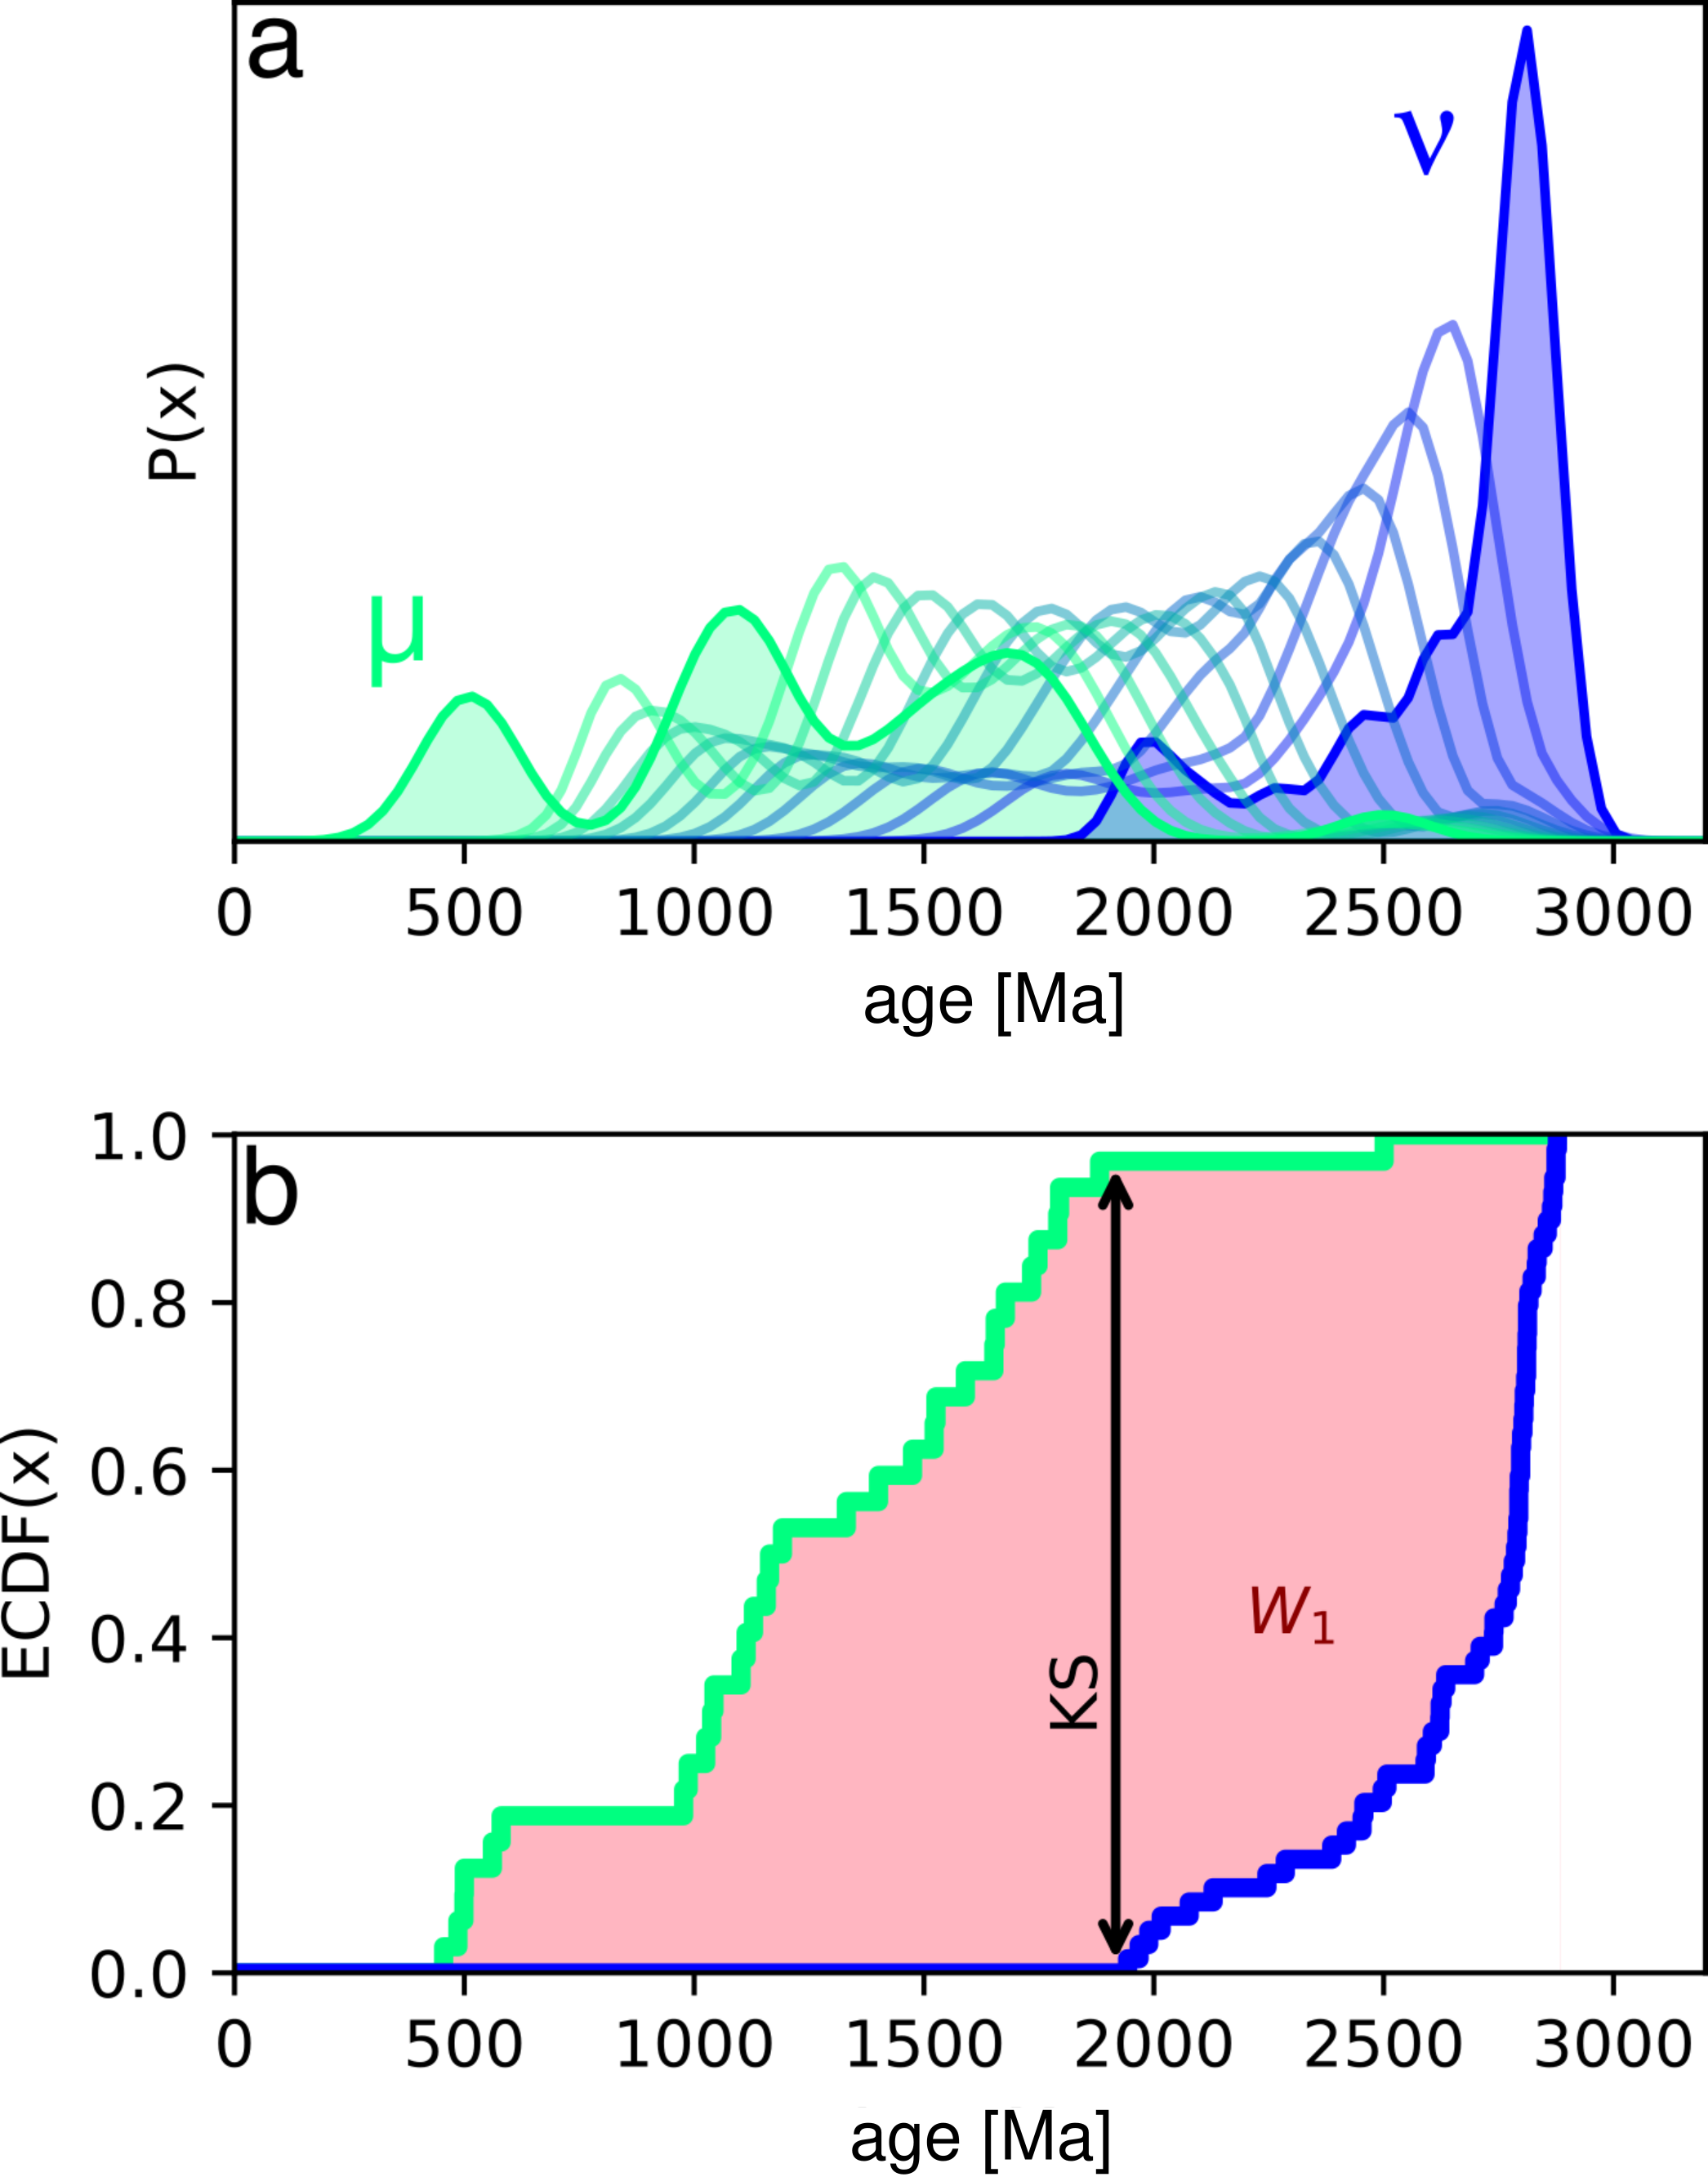
\includegraphics{figures/fig01.png}
    \caption{\textbf{Intuition of the Wasserstein distance.} a) Green and blue filled polygons show two example kernel density estimates of mineral ages from two samples (based on data from \citealt{morton_provenance_2008}) The distributions are labelled $\mu$ and $\nu$ for consistency with Equation \ref{eq:def_1d}. Semi-transparent coloured lines are probability distributions spaced equally in Wasserstein space between $\mu$ and $\nu$ (termed `barycentres'; \citealt{benamou_iterative_2015}). b) Empirical Cumulative Distribution Functions (ECDFs) of the detrital ages used to calculate the distributions shown in panel a, same colours. The first Wasserstein ($W_1$) distance corresponds to the total area between the two ECDFs (shaded pink). The Kolmogorov-Smirnov (KS) distance is the maximum distance between the two ECDFs (black double-headed arrow).}
    \label{fig:intro}
\end{figure}

The Wasserstein distance is a distance metric between two probability measures from a branch of mathematics called `optimal transport'. Optimal transport is often intuited in terms of moving piles of sand from one location to another with no loss or gain of material (e.g., \citealt{villani_topics_2003}). The problem that optimal transport solves is finding the way to transport the sand such that the least sand is moved the least distance. The Wasserstein distance is the cost associated with this most efficient transportation. The association with moving piles of sand is why the Wasserstein distance is often termed the Earth-mover's distance. Figure \ref{fig:intro}a shows an example of how one univariate probability distribution, $\mu$, based on a detrital age spectrum, is transformed into another, $\nu$ according to the optimal transport plan. Elsewhere in the Earth sciences, the Wasserstein distance is increasingly used for solving non-linear geophysical inverse problems (e.g., \citealt{engquist_application_2014,metivier_optimal_2016,sambridge_geophysical_2022}) and has been proposed as a tool for fitting hydrographs \citep{magyar_hydrological_2023}. Full mathematical treatments of the Wasserstein distance and optimal transport are beyond the scope of this paper, but interested readers are referred to \cite{villani_topics_2003} or \cite{peyre_computational_2019}. A geophysical perspective is given in \cite{sambridge_geophysical_2022}. 

\subsection{Formal definition}

We consider two univariate probability distributions $\mu$ and $\nu$ which have cumulative distribution functions (CDFs) $M$ and $N$ respectively. The $p^{\mathrm{th}}$ Wasserstein distance between $\mu$ and $\nu$ is given by: 
\begin{equation}
        W_p(\mu, \nu) = \left(\int_0^1 | M^{-1} - N^{-1} |^p \mathrm{d}t\right)^{1/p}. 
    \label{eq:def_1d}
\end{equation} 
\noindent where $M^{-1}$ indicates the inverse of the CDF $M$ and $0 \leq t \leq 1$ \citep{villani_topics_2003}. Note that this definition of $W_p$ assumes that the cost-function is given by $|x-y|^p$ (e.g., the Euclidean distance where $p=2$), which is the case for most distributional data in geology. In the further special case of $p=1$ (i.e., the \textit{first} Wasserstein distance, $W_1$), Equation~\ref{eq:def_1d} can be re-written simply as: 
\begin{equation}
        W_1 (\mu, \nu) = \int_X | M - N| \mathrm{d}x, 
    \label{eq:def_1d_ecdf}
\end{equation} 
\noindent which is the area between two CDFs (e.g., Figure \ref{fig:intro}b). Recall that the KS-distance between two distributions is the maximum distance between the two corresponding CDFs. Whilst the $W_1$ is easily visualised, we actually use the $W_2$ going forwards as the \textit{squared} distance (i.e., $p=2$) between observations is the standard distance metric in most statistical analyses (e.g., least squares regression). Additionally, $W_2$ decomposes into readily interpretable terms, as discussed below. 

We focus on these univariate instances as they apply to the most common geological distributional data including detrital age distributions and grain size distributions. However, we note that the Wasserstein distance is, in general, multivariate. As a result, some form of the Wasserstein distance could prove useful for analysing a number of other geological datasets such as the geochemical compositions of detrital minerals, or joint U-Pb and Lu-Hf isotope analysis (see \citealt{vermeesch_multidimensional_2023}). Statistics for comparing distributional data in multiple dimensions are increasingly needed \citep{sundell_two-dimensional_2021}. 

Like the KS distance, $W_2$ satisfies the triangle inequality, and as such is a true metric. This property means that classical, as well as metric \& non-metric MDS can be used with a $W_2$ defined dissimilarity matrix. As $W_2$ is sensitive to absolute time differences, metric (or classical) MDS, which seek to preserve absolute distances, may be preferable to non-metric MDS. For the rest of this manuscript, metric MDS is used.  

% \subsection{Formal definition}

% Let $\mu$ and $\nu$ be probability measures defined on spaces $X$ and $Y$ respectively (e.g., the filled polygons in Figure \ref{fig:intro}a). Consider also $c(x,y)$ which is the cost function on $X \times Y$, which can be intuited as the effort expended in moving a grain of sand from location $x$ to location $y$ (Figure \ref{fig:intro}b). We define the \textit{transport plan} as the probability measure $\pi$ on $X \times Y$. The unit measure $d\mathrm{\pi}(x,y)$ is the amount of material transported from location $x$ to location $y$. Given the probability distributions $\mu$ and $\nu$ both sum to one, the marginal sums of $\pi$ must be equal to $\mu$ and $\nu$ i.e, $\int \pi(x,y) \mathrm{d}x = \mu(x)$ and $ \int \pi(x,y) \mathrm{d}y = \nu(y)  $ (Figure \ref{fig:intro}b--d). We define the set of all $\pi$ that fulfil these requirements as $\mathbf{\Pi}$. In the case that $\mu$ and $\nu$ are 1D distributions, each element of $\mathbf{\Pi}$ is a 2D distribution, where integrating along each axis recovers $\mu$ and $\nu$ (e.g., Figure \ref{fig:intro}c). The $p^{th}$ Wasserstein distance between $\mu$ and $\nu$ is defined as: 
% \begin{equation}
%     W_p (\mu, \nu) := \left(\inf\limits_{\pi \in \mathbf{\Pi}(x,y)} \int_{X \times Y} c(x,y)^p d\pi(x,y) \right)^{\frac{1}{p}},
%     \label{eq:definition}
% \end{equation}
% where $\inf$ refers to the infinum (or greatest lower bound) of a set \citep{kantorovich_translocation_1942}. In other words, it is the total cost associated with the \textit{optimal} transport plan, $\pi$, which involves moving the least amount of material, $\mathrm{d}\pi(x,y)$, the least amount of distance, $c(x,y)$. 

\subsection{Decomposition}

A particularly useful property of $W_2$ between two univariate distributions is that it can be decomposed in terms of the differences between the two distributions' location, spread and shape. \cite{irpino_optimal_2007} show that: 
\begin{equation}
    W^2_2(\mu,\nu) = \overbrace{(\bar{\mu} - \bar{\nu})^2}^{Location} + \overbrace{(\sigma_{\mu} - \sigma_{\nu})^2}^{Spread} + \overbrace{2\sigma_{\mu}\sigma_{\nu}(1-\rho^{\mu \nu})}^{Shape},
    \label{eq:decomposition}
\end{equation}
where $\bar{\mu}$ is the mean of $\mu$, $\sigma_{\mu}$ is the standard deviation of $\mu$ and $\rho^{\mu\nu}$ is the Pearson correlation coefficient between the quantiles of the distributions $\mu$ and $\nu$. These three terms also accord with, qualitatively, how as geologists we might compare two distributions. 

\subsection{Discrete data}

Most distributional data in the Earth sciences do not, in raw form, follow continuous probability distributions. Instead, samples may be discrete sets of observations, e.g., lists of individual mineral ages. The above formulations can be easily applied to such cases by describing the probability functions $\mu$ and $\nu$ as weighted sums of $\delta$ functions. For example, let us consider two samples $x_m$ and $x_n$ with $p$ and $q$ numbers of observations respectively: 

\begin{equation}
        \mu = \sum^p_i m_i \delta_{x_m}, \quad
        \nu = \sum^q_i n_i \delta_{x_n}
\end{equation}

where $m$ and $n$ are weight vectors, such that $\sum m_i = \sum n_i = 1$. In most geological cases these weights would be uniform, $m_i = 1/p;~ n_i = 1/q$, giving each observation within a sample equal weight. 
In this scenario, $M$ and $N$ are the familiar empirical cumulative distribution functions (ECDF), given as a series of step functions (e.g., Figure \ref{fig:intro}b). 

\subsection{A synthetic example}

\begin{figure}
    \centering
    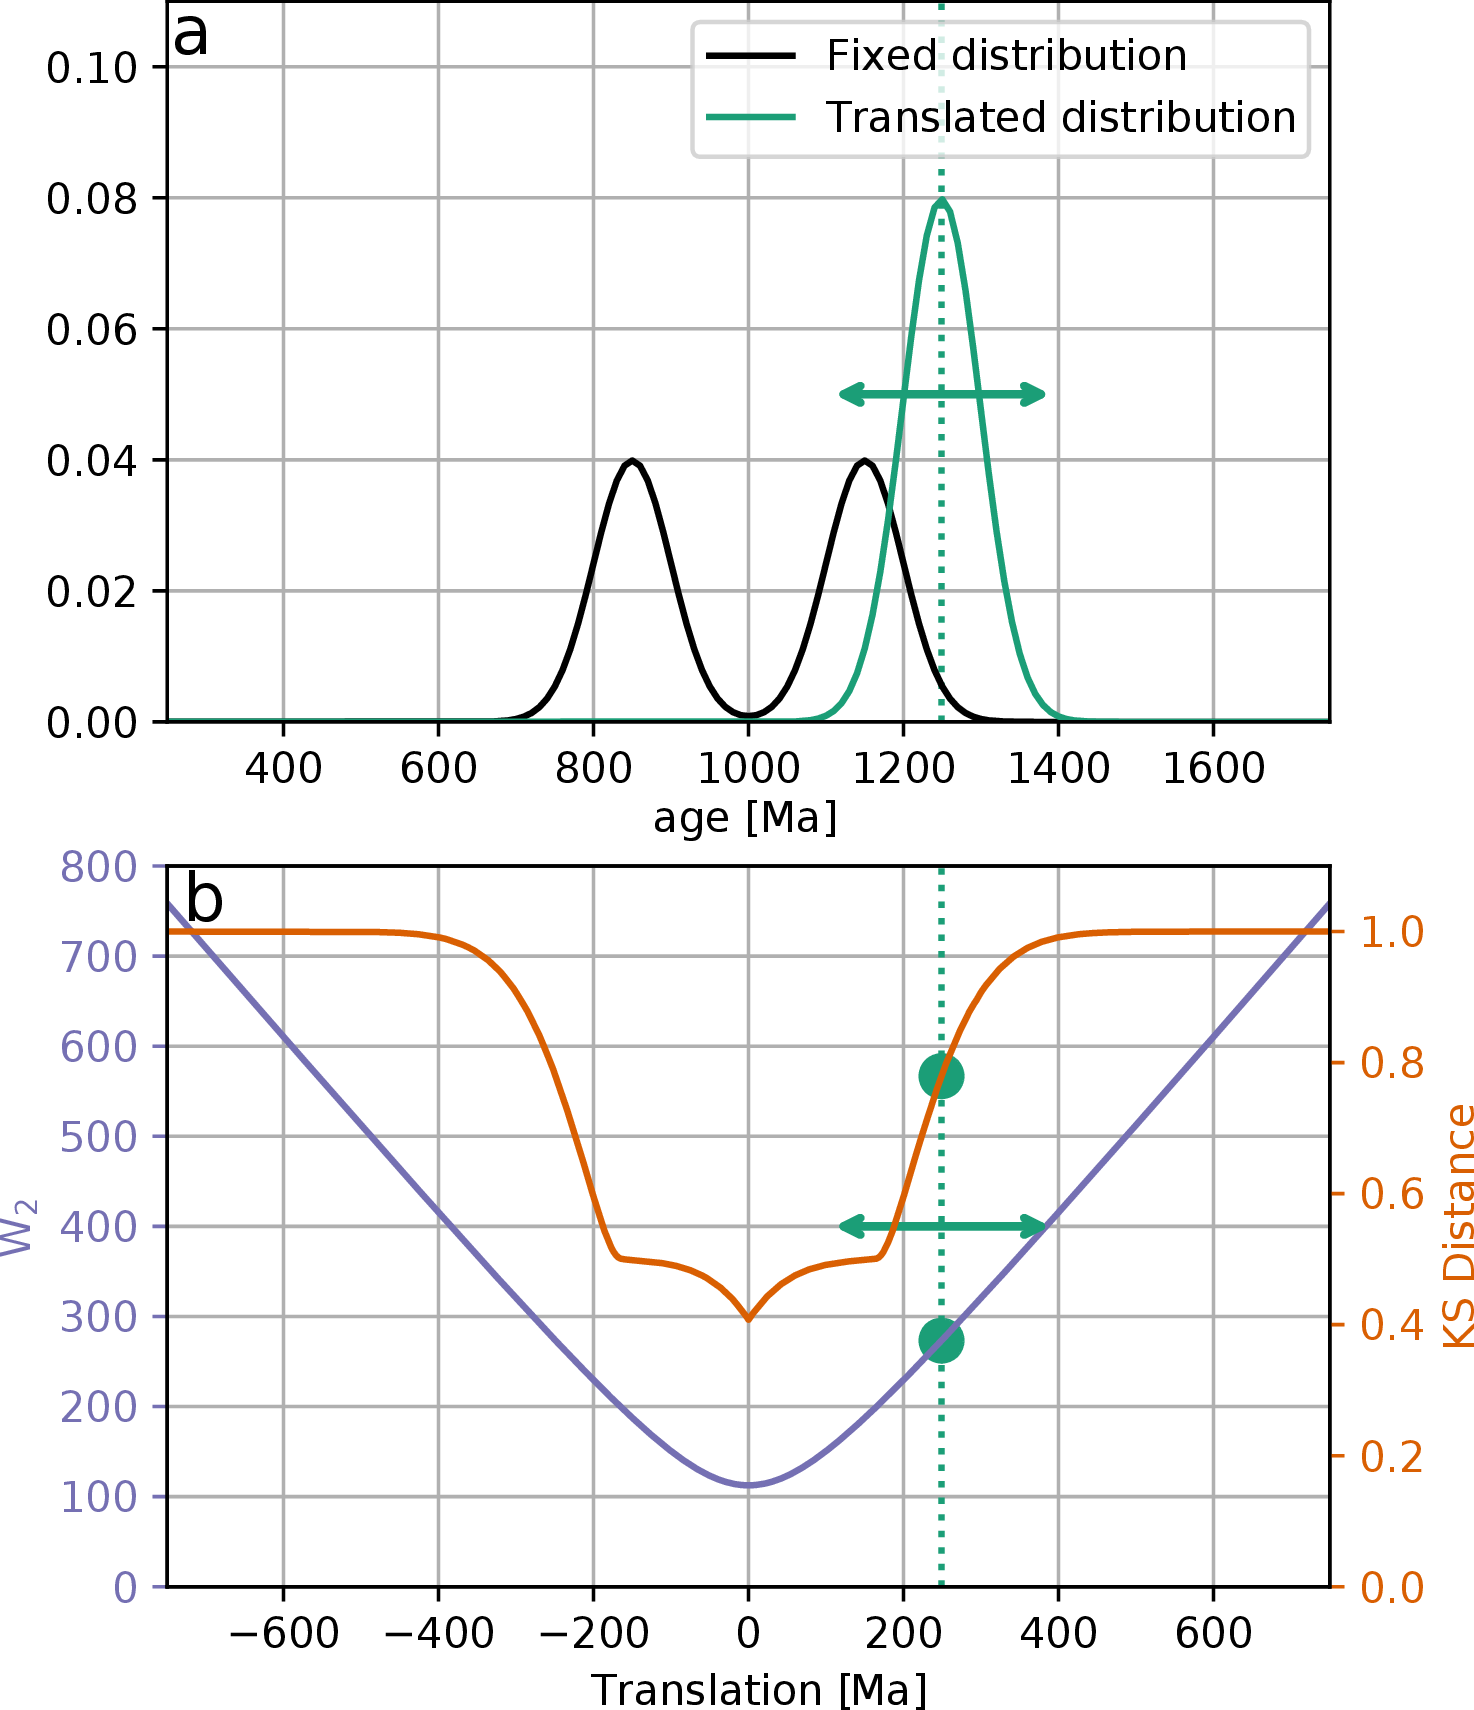
\includegraphics[scale=0.65]{figures/fig02.pdf}
    \caption{\textbf{Comparing the Wasserstein distance to the Kolmogorov-Smirnov distance.} a) Two synthetic probability density functions, modelled on U-Pb age spectra. The black bimodal distribution is fixed at 1000 Ma, and the green unimodal distribution is translated along the time axis. b) For each translated distribution, we calculate the KS-distance (red line) and $W_2$ (blue line). The green dashed line and circles indicate values associated with the location of the green distribution shown in panel a.}
    \label{fig:translation}
\end{figure}

To demonstrate the intuition of $W_2$ we explore a simple synthetic example. We consider two probability density functions of mineral ages: a bimodal distribution and a unimodal distribution, both constructed from Gaussians with the same scale (Figure \ref{fig:translation}a). We fix the bimodal distribution at 1000~Ma, but translate the unimodal distribution along the time axis. For each translated distribution we calculate both the KS-distance and $W_2$. Figure \ref{fig:translation}b displays the behaviour of both distances under this scenario. The KS-distance shows an unexpectedly complex response containing a series of steps, as the peaks of the distributions align and misalign. At around $\pm{400}$~Ma, once the distributions stop overlapping, the KS-distance plateaus at its maximum value of 1. By contrast, $W_2$ increases monotonically with increasing distance. Away from the origin, $W_2$ approximates a linear function of the amount of translation, as is predicted from Equation \ref{eq:decomposition}. At the origin, the non-zero value of $W_2$ is the cost of turning the unimodal distribution into the bimodal distribution without translation. 

We argue that the behaviour of $W_2$ is more geologically intuitive than the KS-distance under this scenario. It is useful geological information if two distributions differ in their means by 400, 500 or 1000 Ma, but if the distributions do not overlap, the KS-distance is insensitive to this. The Wasserstein distance is, by contrast, sensitive to the absolute offset between non-overlapping distributions. Additionally, the stepped response of the KS-distance under translation is undesirable. Under the simple operation of translating a unimodal distribution, we would expect our dissimilarity to increase at a constant, or at least predictable (e.g., quadratic) rate. The change of the KS-distance with translation is, unintuitively, non-linear. By contrast, the $W_2$ increases linearly with respect to translation.

\DIFaddbegin \DIFadd{We reiterate that at a translation of 0 Ma, $W_2$ (and the KS distance) is still non-zero, reflecting the fact that even when the average ages are aligned, the shapes of the uni-modal and bi-modal distributions do not match. This illustrates the tendency of $W_2$ in geochronological data to prioritise aligning the average ages of distributions }\textit{\DIFadd{before}} \DIFadd{considering matching individual peaks. Such behaviour contrasts with approaches that seek to only match probability peaks neglecting any information of absolute ages (e.g., \mbox{%DIFAUXCMD
\citealt{saylor_quantifying_2016}}\hspace{0pt}%DIFAUXCMD
).
}

\DIFaddend % \section{Use of Wasserstein distance in multi-dimensional scaling}

% \begin{figure}[!h]
%     \centering
%     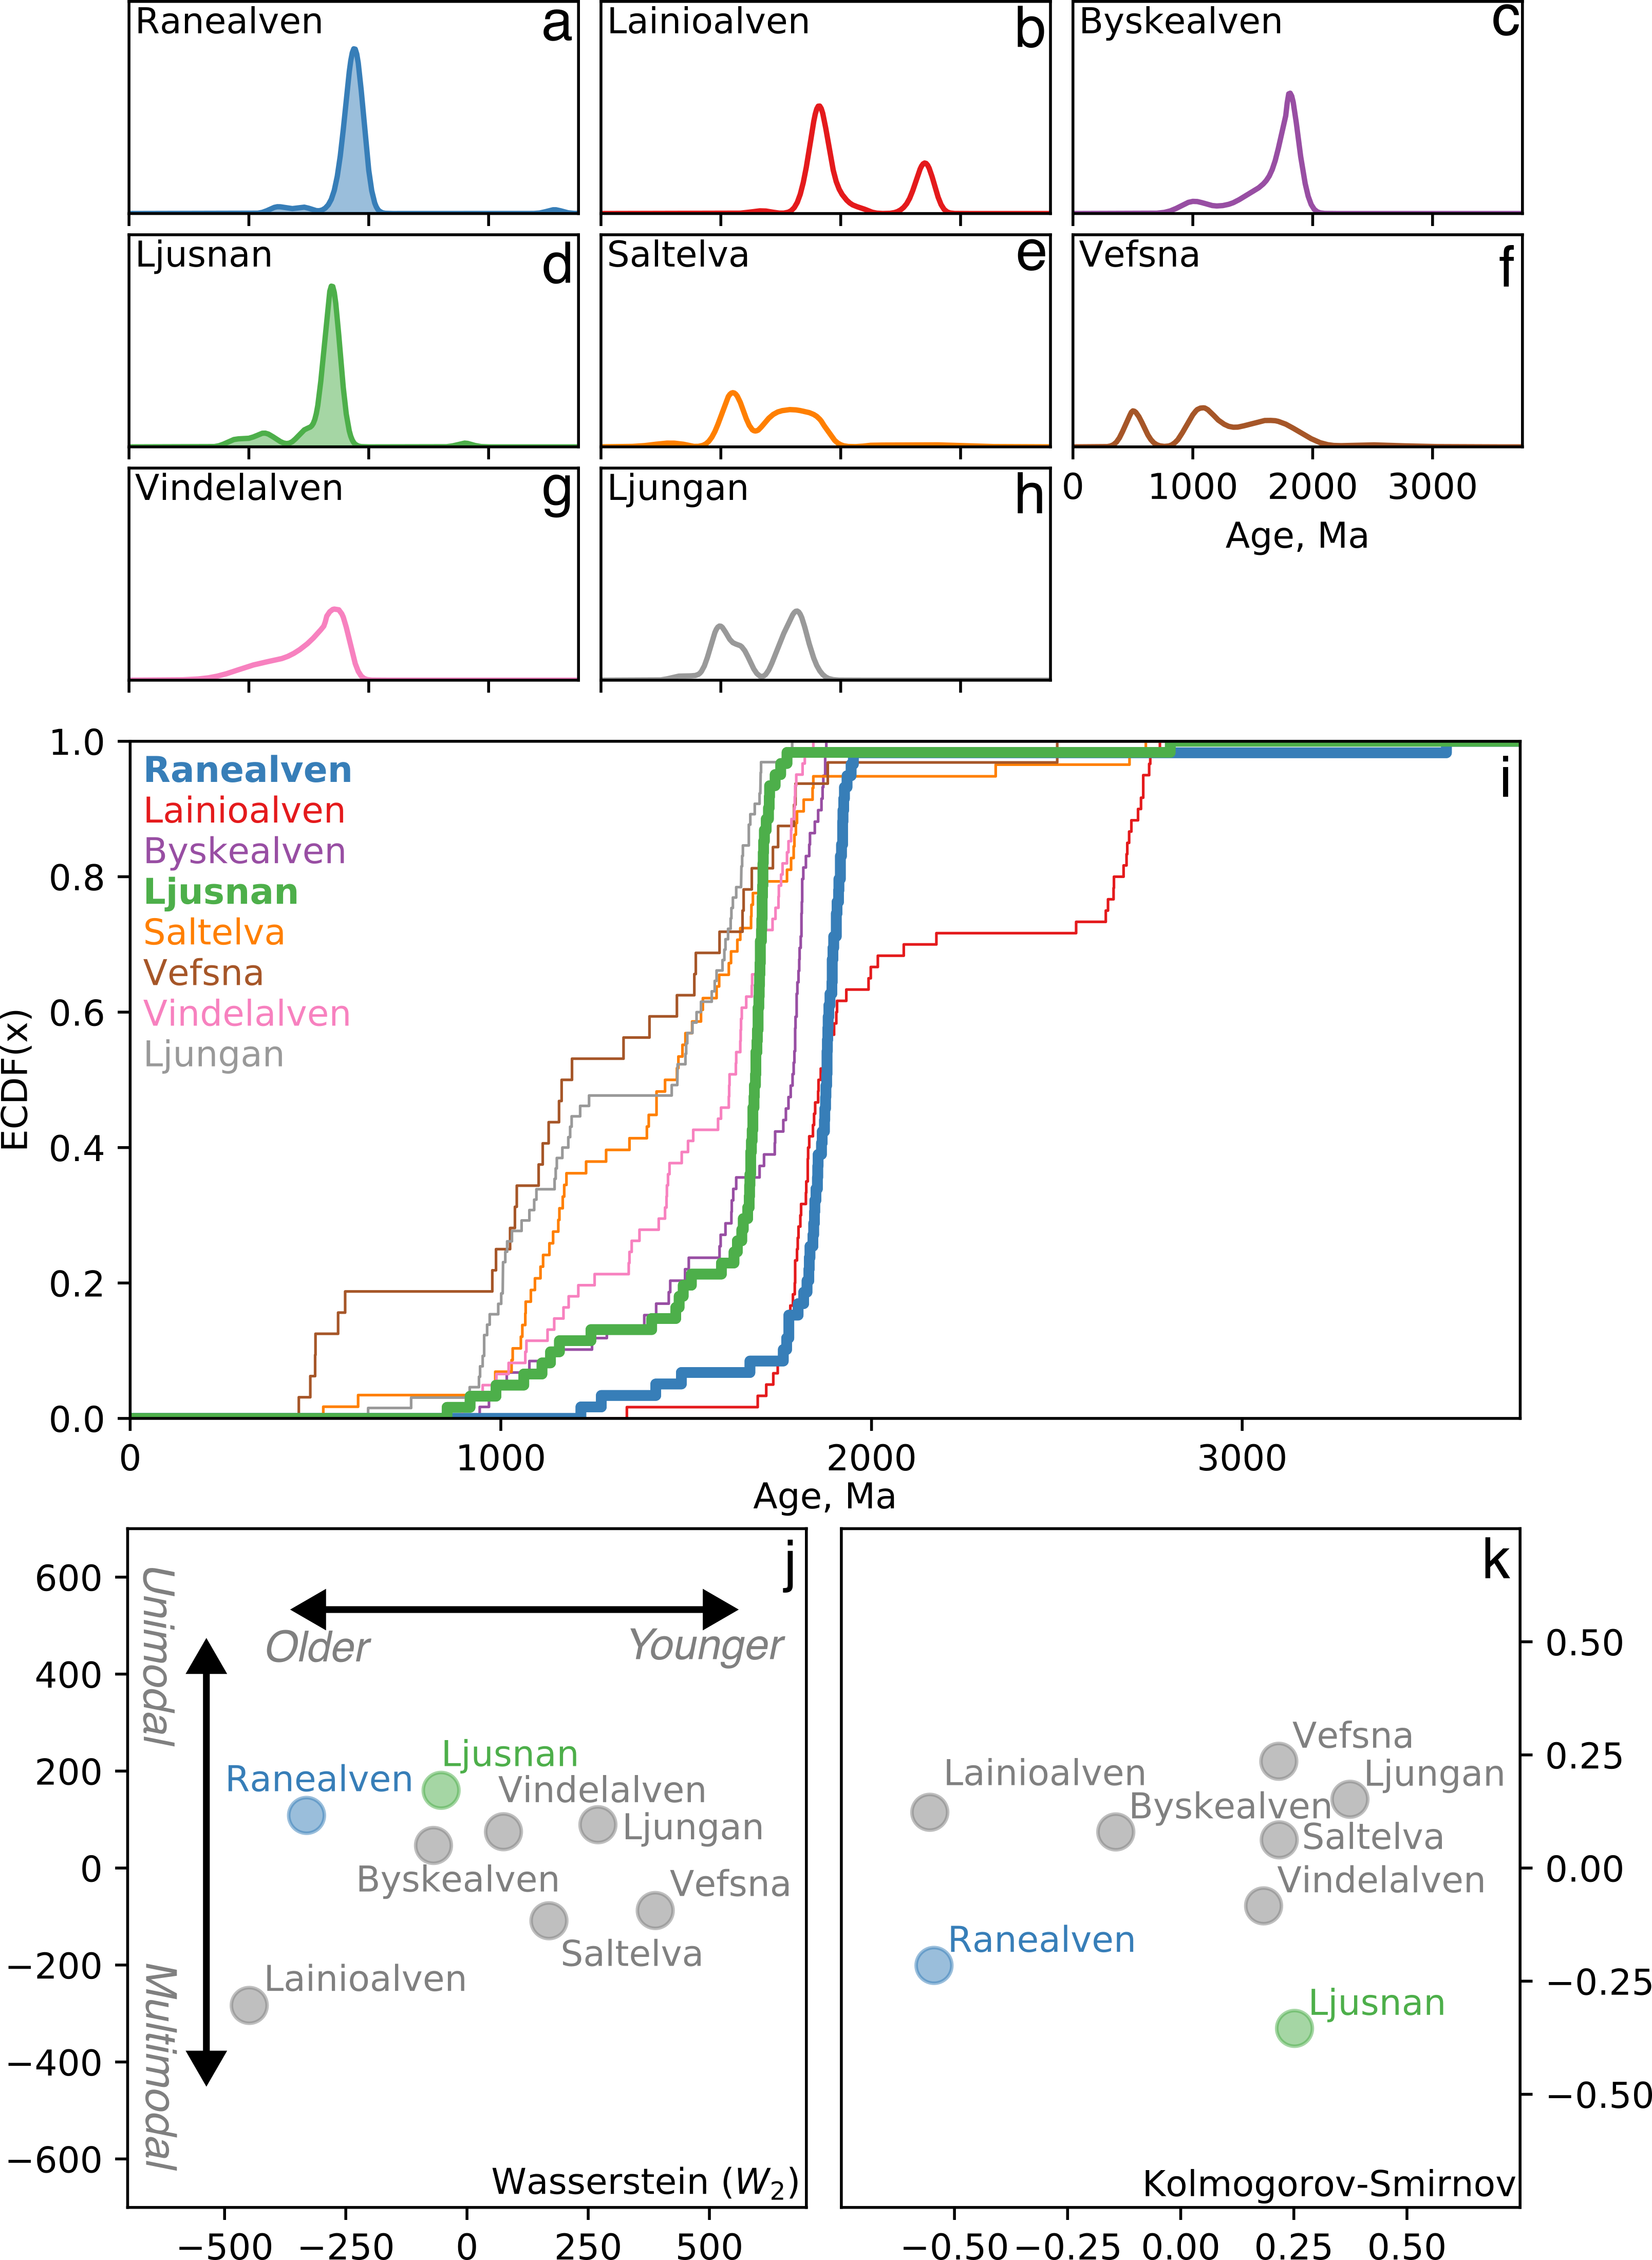
\includegraphics[scale=0.75]{figures/fig03.png}
%     \caption{\textbf{Analysing detrital zircon U-Pb ages using the Wasserstein distance.} a--h) Kernel Density Estimates (KDEs) of zircon U-Pb ages from modern sand gathered in Scandinavian rivers by \cite{morton_provenance_2008}. Sampled river names are indicated in the upper left corners of the plots. `Ranealven' and `Ljusnan' samples are filled in and highlighted in panels i--k. KDEs generated using a Gaussian kernel with adaptive bandwidth \citep{shimazaki_kernel_2010}. i) Empirical Cumulative Distribution Functions (ECDFs) for each zircon age population. j) Multi-Dimensional Scaling (MDS) map for zircon populations calculated using $W_2$ as a dissimilarity metric. Note the closeness of `Ranealven' and `Ljusnan'. k) MDS map of same samples but using KS-distance. Note the distance separating `Ranealven' and `Ljusnan'.}
%     \label{fig:mds}
% \end{figure}

% We now use $W_2$ to analyse a real dataset of zircon U-Pb ages from Scandinavian river sediments gathered by \cite{morton_provenance_2008}. This dataset contains eight samples displayed as kernel density estimates in Figure~\ref{fig:mds}a--h and ECDFs in Figure \ref{fig:mds}i. This data is provided in \texttt{.csv} format at the code repository (\url{https://github.com/AlexLipp/detrital-wasserstein/}). Full geological details of the provenance of these samples can be found in \citet{morton_provenance_2008}, briefly summarised here. The sampled rivers drain two major geological provinces: the Fennoscandian Shield (Byskeälven, Raneälven, Lainioälven and Ljusnan) and the Caledonian Nappe Domain (Salteva, Vefsna, Vindelälven and Ljungan). The Shield primarily consists of paleoproterozoic crystalline, volcanic and metasedimentary rocks, with a minor outcrop of Archean basement \citep{gaal_outline_1987} The Caledonian Nappe domain comprises mostly of meta-sedimentary units deposited on the Baltica passive margin which were emplaced atop the shield in the Paleozoic \citep{roberts_scandinavian_2003}. The number of grains for each sample in this study is relatively small (maximum $n=66$) compared to the numbers that are generally sought. However, given we seek to compare given populations of mineral ages, rather than characterise a known distribution given a finite population of ages, the small sample size should not greatly impact our results.   

% Here, we use MDS to jointly compare all samples \citep{vermeesch_multi-sample_2013}. One of the desirable properties of the Wasserstein distance is that it fulfils the metric requirements, just like the KS-distance \citep{villani_topics_2003}. Therefore, $W_2$ dissimilarity measures can be analysed by classical as well as non-metric MDS algorithms \citep{vermeesch_multi-sample_2013}. The MDS `maps' calculated by non-metric MDS, using both $W_2$ and the KS-distance, are shown in Figure \ref{fig:mds}j--k. We investigate whether the KS map or the $W_2$ map shows greater geological meaning.

% We initially focus on two samples: Ranealven (Figure \ref{fig:mds}a) and Ljusnan (Figure \ref{fig:mds}d). These two samples have very similar distribution shapes with one prominent peak, and a smaller younger peak. However, the prominent peak is slightly offset between the two distributions such that there is little overlap. This feature is well shown in the ECDF plot in Figure \ref{fig:mds}h. As there is limited overlap between them, the KS-distance between these two visually similar distributions approaches its maximum value of 1. As a result, when MDS is applied to the dataset using the KS-distance these two samples are, counter-intuitively, widely separated (Figure \ref{fig:mds}k). By contrast, when using $W_2$, the samples are close together (Figure \ref{fig:mds}j). 

% The $W_2$ MDS projection also accords well with the actual geological provenance of these samples with samples of the same provenance being grouped together. Whilst the axes of an MDS plot hold no inherent meaning, we can interpret relative positions on the map in terms of distributions' shapes and average ages. The horizontal axis, in this case, appears approximately coincident with the average age of the samples, with the samples to the left being generally older than those on the right. For example, the peak of Ljusnan is younger than that of Ranealven. In addition, the sample containing the most recent grains, Vefsna, is the furthest to the right. Contrastingly, Lainioalven, which uniquely drains Archean rocks, is the furthest to the left. Similarly, the vertical axis correlates approximately with distribution shape. Salteva \& Vefsna have a broad, multimodal distribution and are placed towards the bottom of the map. Conversely, Ranealven \& Ljusnan are largely unimodal. Byskealven \& Vindelalven lie between these two endmembers and this is reflected in the MDS map. Given that $W_2$ can be deconvolved into interpretable statistics (Equation \ref{eq:decomposition}) it is not surprising that the MDS maps produced can also be discussed in these terms. 

\section{Discussion}

As stated above, the most appropriate dissimilarity metric to use will depend on the \DIFdelbegin \DIFdel{data being analysed and the }\DIFdelend scientific question being answered. In general, the Wasserstein distance is most appropriate when absolute differences along the time axis (or more generally, the x-axis) provide useful information to solving the geologic problem. The KS distance however is more appropriate when the size of the time differences between peaks is not relevant. Both the KS distance and the $W_2$ are calculated in terms of differences between ECDFs. Due to these similarities in construction, in many cases the results from using the KS and $W_2$ are, encouragingly, similar. One exception is whether ages are log transformed prior to analysis. Because the KS distance considers only the order of the ages, it will be the same whether a log transform is used or not. $W_2$ however will be different, and will consider \textit{relative} not absolute age differences.  Such an example is discussed below (Figure \ref{fig:Wobus}). 

Here we discuss a variety of realistic scenarios where the KS and $W_2$ may result in different interpretations. In each, we evaluate the advantages and disadvantages of using $W_2$ or KS. These case-studies can be used to determine which metric is most appropriate for a particular scenario. 

\subsection{Discriminating contributions from discrete endmembers}

\begin{figure}
    \centering
    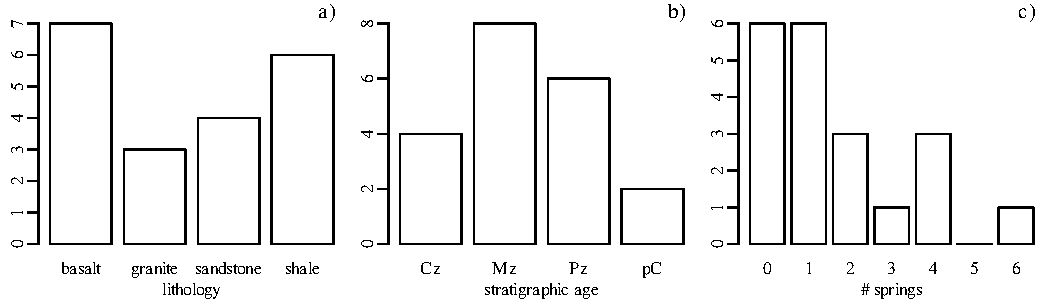
\includegraphics[scale=0.8]{figures/discrete.pdf}
    \caption{\textbf{Mixing of discrete endmembers} a) Three theoretical, unimodal source age distributions with peaks at 10, 20 and 100 Ma, and two mixture samples. Sample 1 is an equal mixture of X and Y and Sample 2 a mixture of Y and Z. b) Metric MDS map of the three sources and the mixtures using $W_2$ distance \DIFaddbeginFL \DIFaddFL{(stress = 0.05)}\DIFaddendFL . c) Same as panel b for KS distance \DIFaddbeginFL \DIFaddFL{(stress = 0.05)}\DIFaddendFL . This is a scenario where KS distance may be preferable to $W_2$.}
    \label{fig:discrete}
\end{figure}

We first consider a scenario where the samples are assumed to be mixtures, in differing proportions, of some known or unknown fixed endmembers. This situation is one where absolute distance along the time-axis is not relevant, as the nature of the endmembers is not sought, simply their relative contributions to a set of mixtures. Instead, it is \textit{vertical} differences in the probability at a given age that is relevant. The KS distance, which is sensitive to such vertical differences in age distributions is better suited for this than $W_2$. Indeed, in such a scenario the $W_2$ can result in some unintuitive behaviour. 

For example, let us consider three unimodal potential sediment sources, as shown in Figure \ref{fig:discrete}a. We now consider two mixture samples. The first is an equal mixture of X and Y, and the second an equal mixture of Y and Z (bottom two plots, Figure \ref{fig:discrete}a). Geologically, we would expect these samples to be about half as similar to the two source endmembers. However, a $W_2$ MDS map identifies these samples as being removed from their two endmembers \DIFdelbegin \DIFdel{\ref{fig:discrete}b}\DIFdelend \DIFaddbegin \DIFadd{(Figure \ref{fig:discrete}b)}\DIFaddend . Additionally, because of the absolute time difference between Source Z and the other sources, Sample 2 is treated as a considerable outlier. The KS distance performs better here, placing the mixtures approximately halfway between the expected endmembers. However, in such a well defined mixing scenario as this, methods such as endmember mixture modelling may be more appropriate than statistical dimension reduction (e.g., \citealt{weltje_end-member_1997,sharman_sediment_2017,dietze_grain-size_2019}).

\subsection{Temporally varying source age distributions}

\begin{figure}
    \centering
    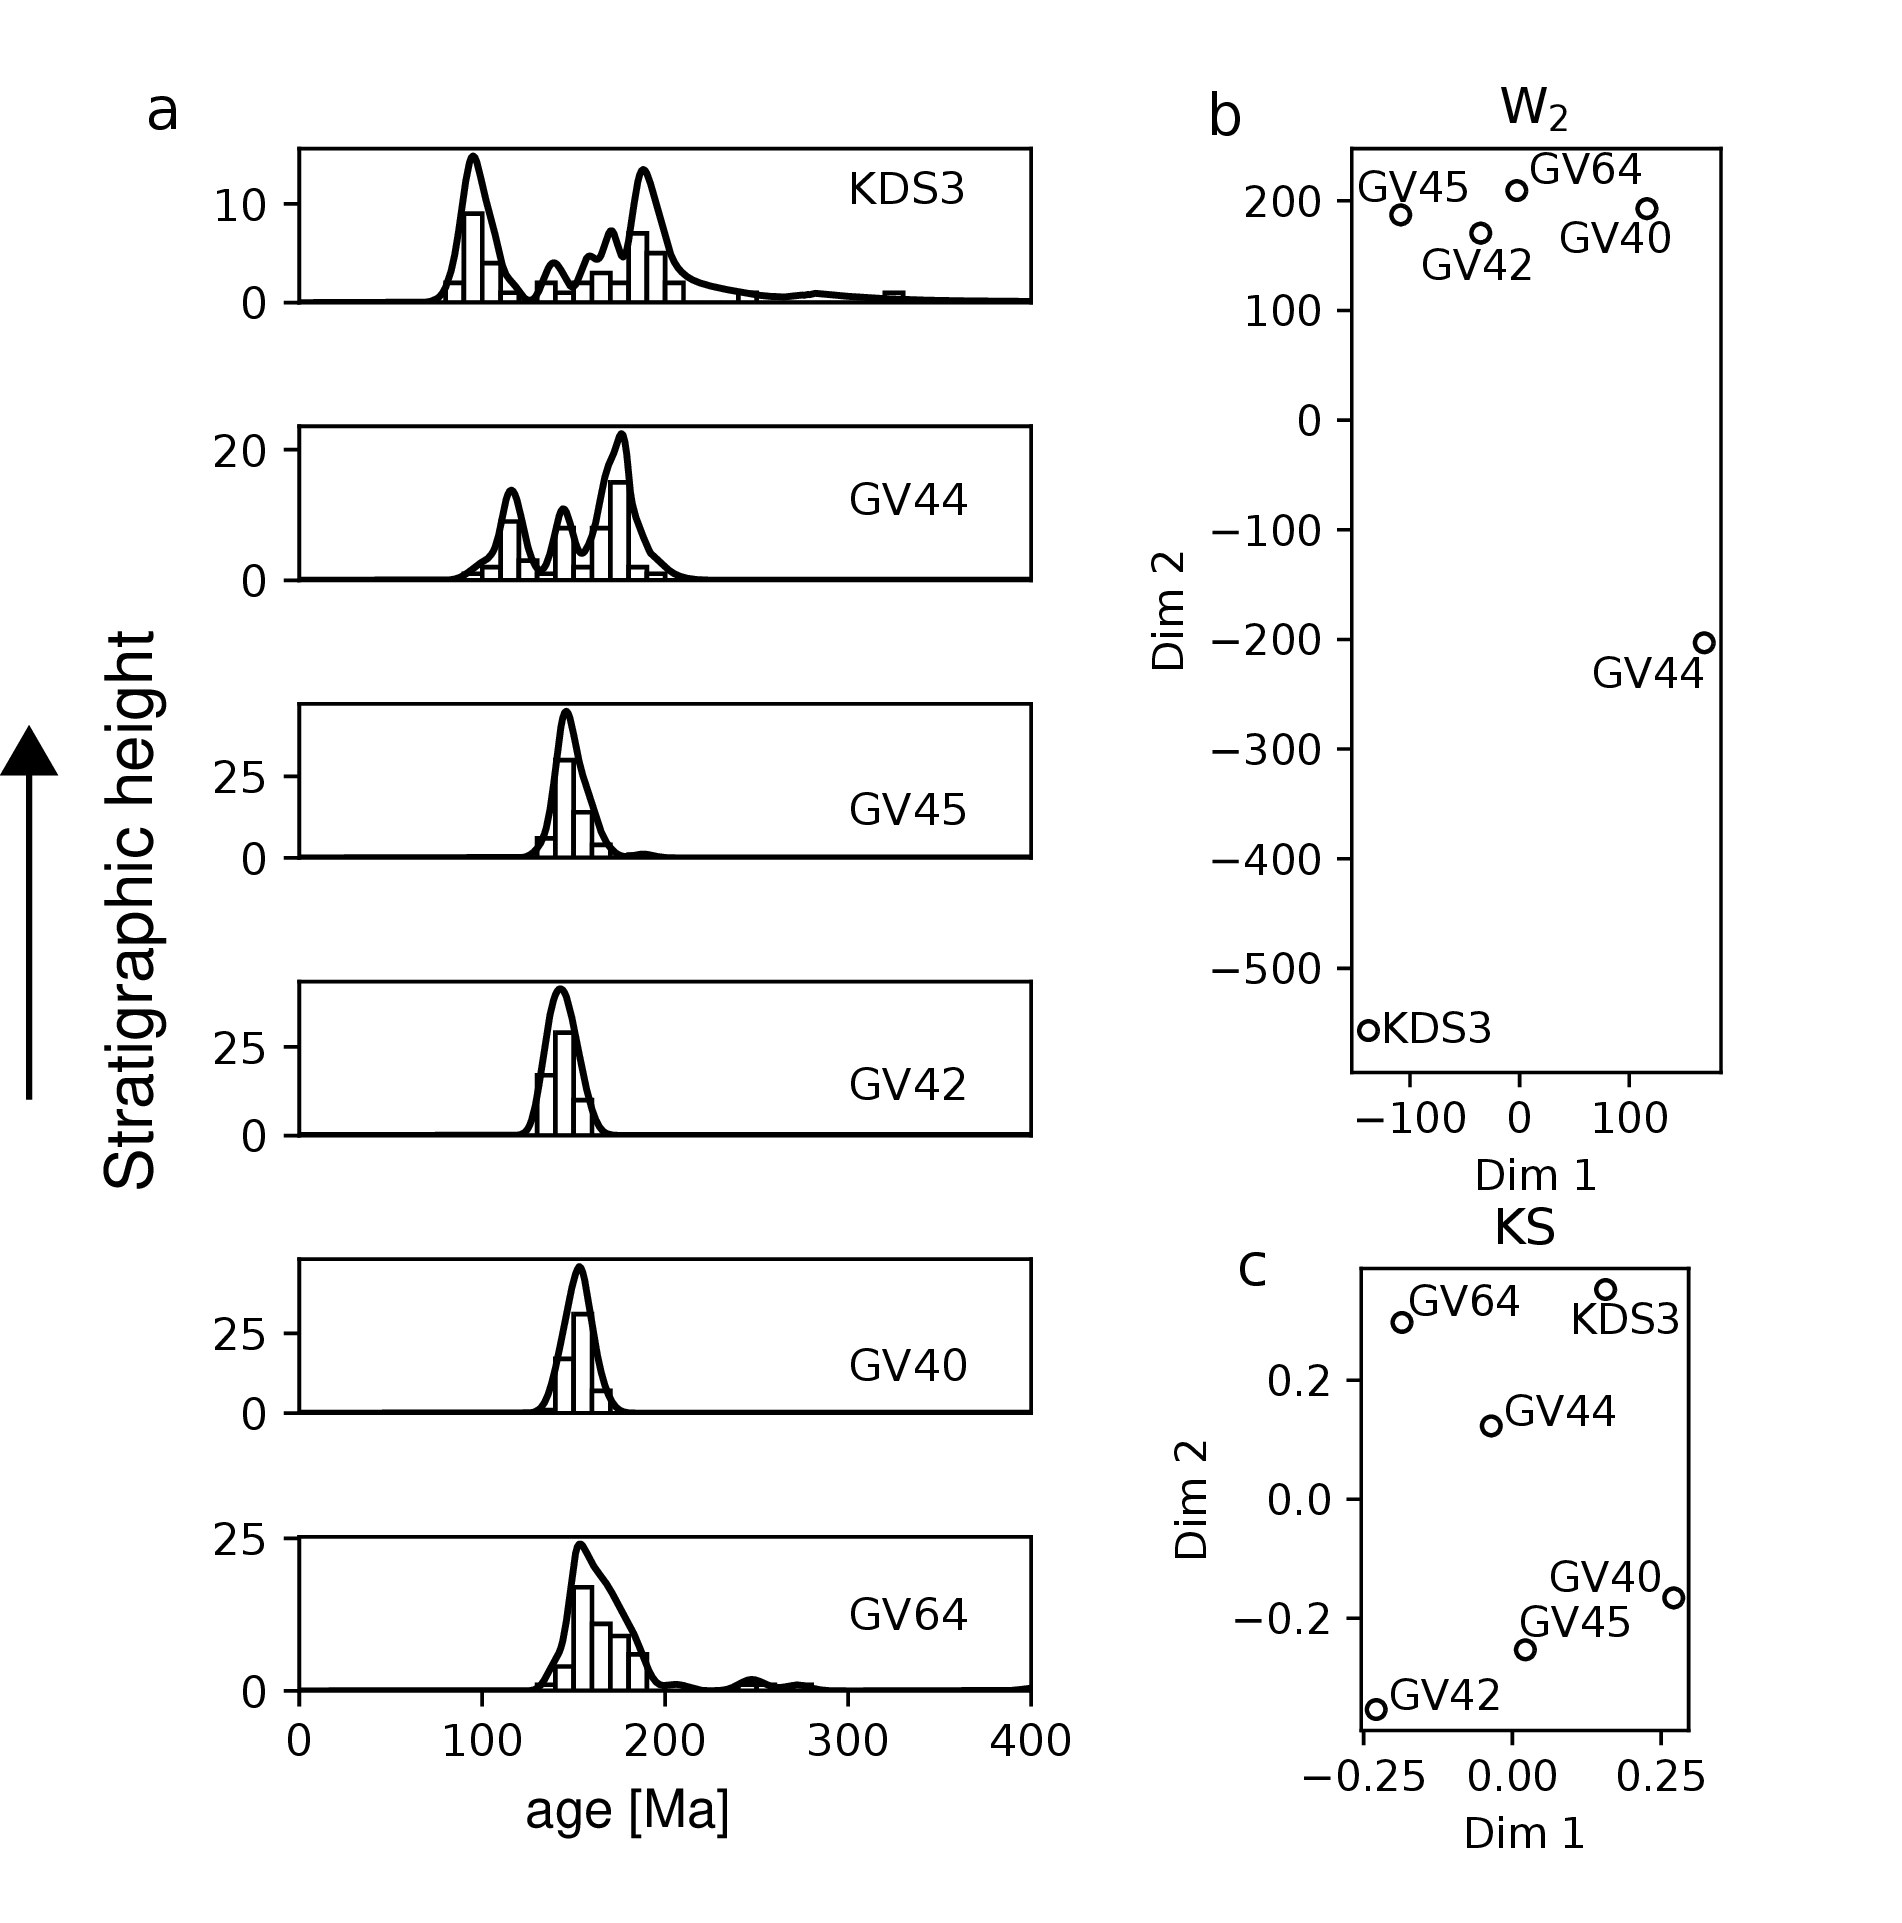
\includegraphics[scale=0.7]{figures/surpless.pdf}
    \caption{\textbf{Temporally evolving source distributions.} a) KDEs and histograms for zircon age distributions for samples from Cache Creek section across Great Valley Group, arranged in stratigraphic order \citep{degraaff-surpless_detrital_2002}. b) MDS map using $W_2$ for data shown in panel a \DIFaddbeginFL \DIFaddFL{(Stress = 0.28)}\DIFaddendFL . c) Same as b using KS distance \DIFaddbeginFL \DIFaddFL{(Stress = 0.18)}\DIFaddendFL . In this scenario, the results from $W_2$ are preferable. } 
    \label{fig:surpless}
\end{figure}

In contrast, scenarios where the shape of sediment source age distributions evolves in space and time are well suited to using $W_2$. This is because $W_2$ considers all parts of a distribution, whereas the KS only compares one point, the location of maximum ECDF separation. For example, Figure \ref{fig:surpless} displays detrital zircon age distributions gathered by \citet{degraaff-surpless_detrital_2002} from sediments from a section (Cache Creek) across the Great Valley Group in California, USA. The age populations are shown as KDEs and histograms, in stratigraphic order, in Figure \ref{fig:surpless}a. The uppermost samples show an increasingly broad distribution than the lower four unimodal samples. \citet{degraaff-surpless_detrital_2002} attribute this trend, \textit{inter alia}, to expanding sediment source areas. 

Figures \ref{fig:surpless}b--c display MDS maps calculated using $W_2$ and KS respectively. The $W_2$ map clearly identifies the stratigraphic order of the samples by the changing distribution shape. Additionally, it clusters the four unimodal samples together. By contrast, the KS map does not identify the stratigraphic trend, locating the lowermost stratigraphic sample GV64 with the uppermost samples KDS3 and GV44. We conclude then that the $W_2$ has better captured the geological information in this scenario.

\subsection{Thermochronology}

In thermochronology, age distributions shift along the time-axis according to thermal signals (e.g., exhumation). In many thermochronological studies, we may seek to characterise how such a signal evolves in space and time. For this question absolute distance along the time-axis is useful information and so the $W_2$ may be more effective than the KS distance. For example, \citet{wobus_has_2003} use $^{40}$Ar/$^{39}$Ar detrital mica thermochronometry to explore spatially varying exhumation along a spatial transect in the Himalaya. The KDEs of the samples are shown in Figure \ref{fig:Wobus}a arranged south to north. The southern samples (WBS1, WBS2, WBS3, WBS8) show old exhumation signals, but a dramatic shift to younger ages is observed north of a distinct physiographic transition. MDS maps of these samples are shown using the KS distance and $W_2$ in Figures \ref{fig:Wobus}b--c respectively. As there is limited overlap between the samples, the KS distance struggles to capture the NS progression in exhumation age. Whilst the physiographic division is found, it weights it equally to variation within one cluster. By contrast, the $W_2$ map correctly identifies the simple temporal and geographical trend of the samples from south to north. 

\begin{figure}
    \centering
    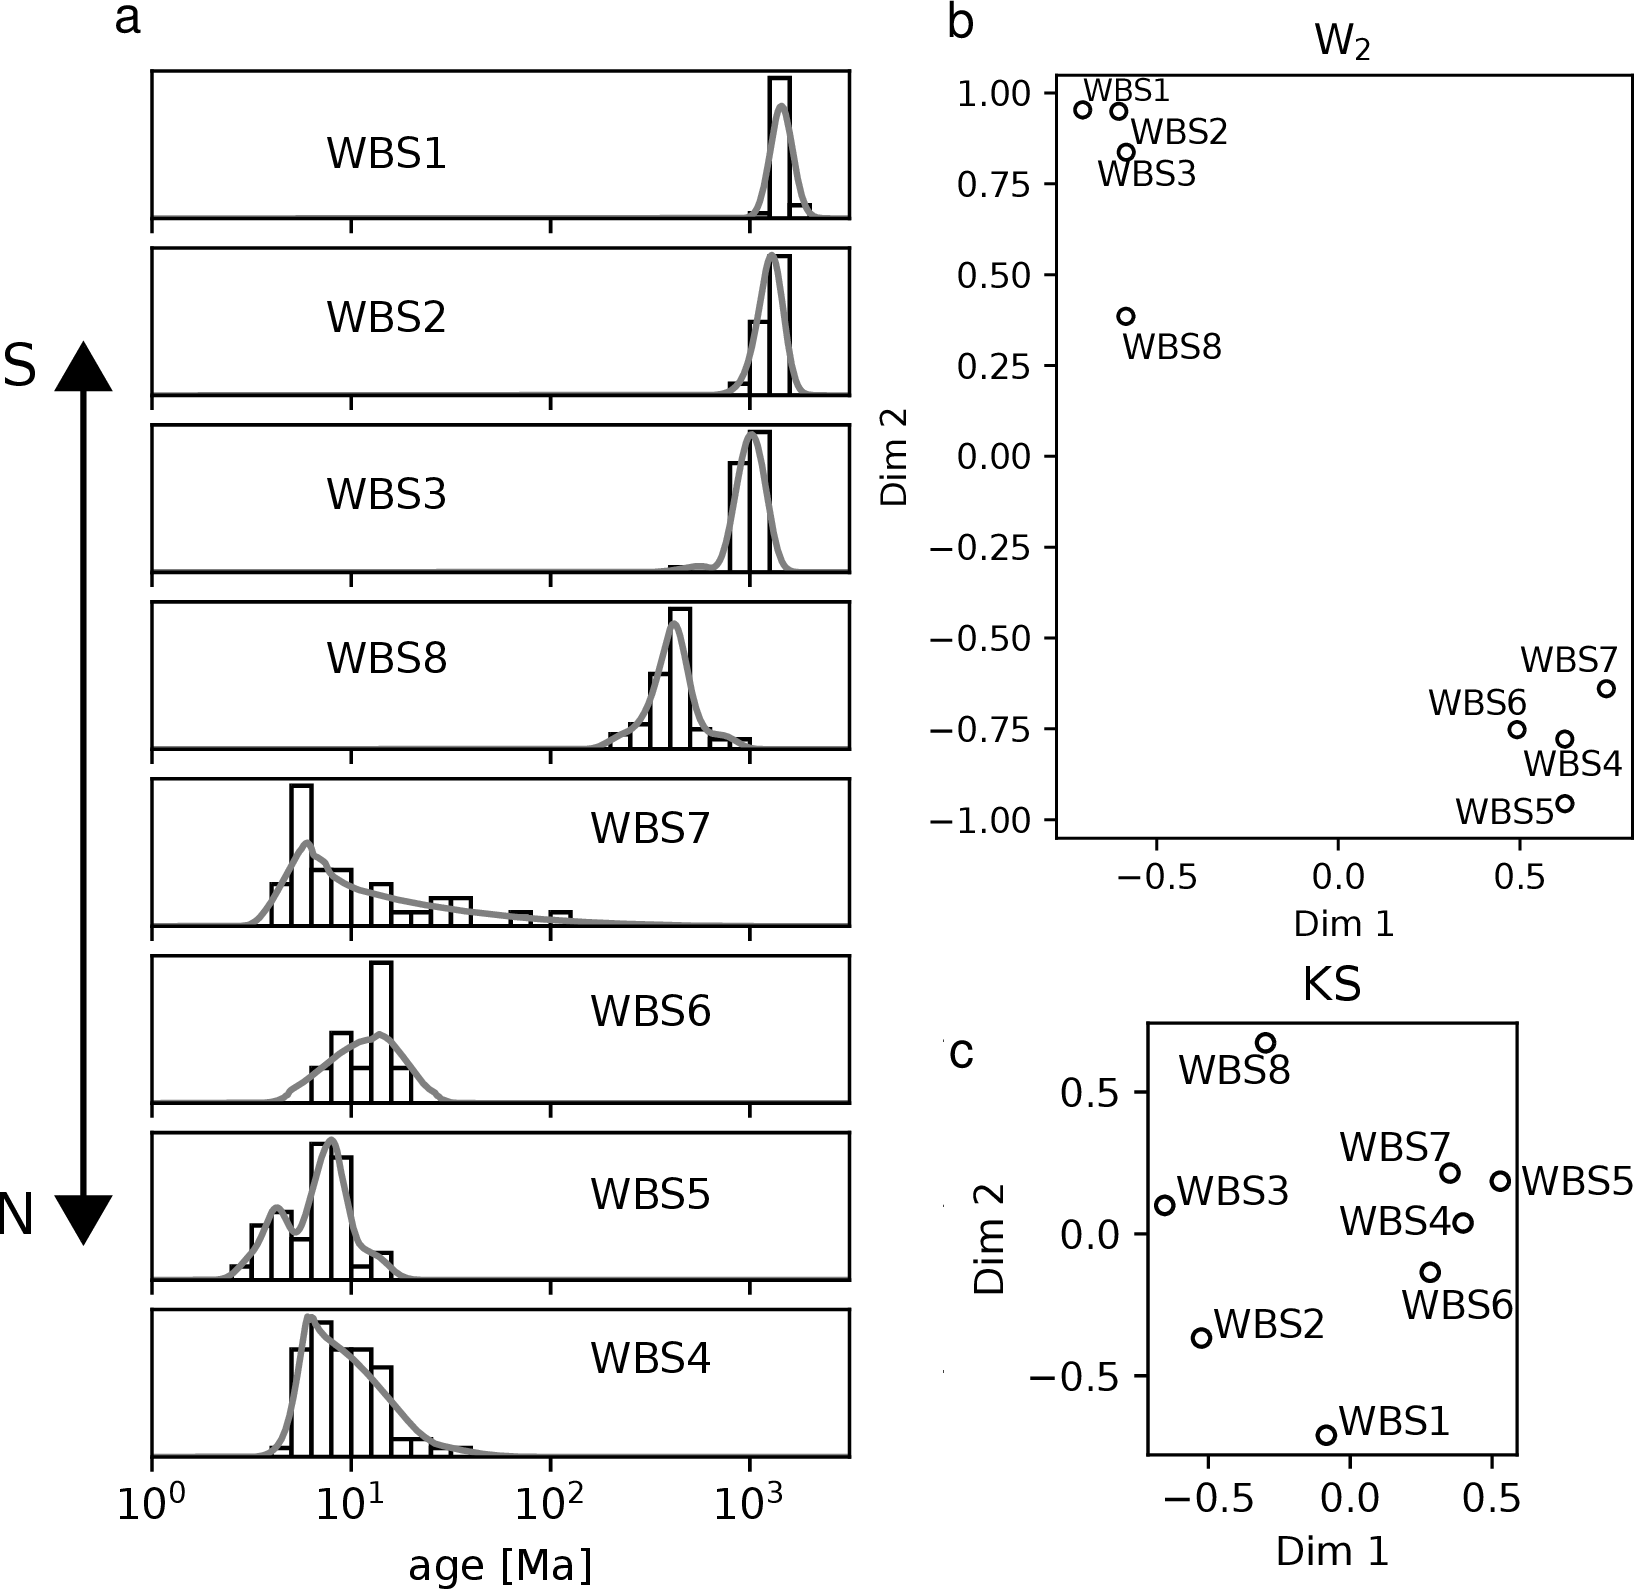
\includegraphics[scale=0.8]{figures/wobus.pdf}
    \caption{\textbf{Analysing thermochronological data using $W_2$ and KS distances.} a) KDEs for a detrital mica \textsuperscript{40}Ar/\textsuperscript{39}Ar dataset of \citet{wobus_has_2003} arranged from south to \DIFdelbeginFL \DIFdelFL{south }\DIFdelendFL \DIFaddbeginFL \DIFaddFL{north }\DIFaddendFL across a physiographic transition of the central Himalaya in Nepal. Note the logarithmic scale. b) The MDS configuration using $W_2$, following a log transform \DIFaddbeginFL \DIFaddFL{(stress = 0.02)}\DIFaddendFL . c) MDS map using KS statistic \DIFaddbeginFL \DIFaddFL{(stress = 0.18)}\DIFaddendFL . In this example, $W_2$ performs better than the KS distance at identifying the geographic trend.}
    \label{fig:Wobus}
\end{figure}

\subsection{Combining data from multiple laboratories}

\begin{figure}
    \centering
    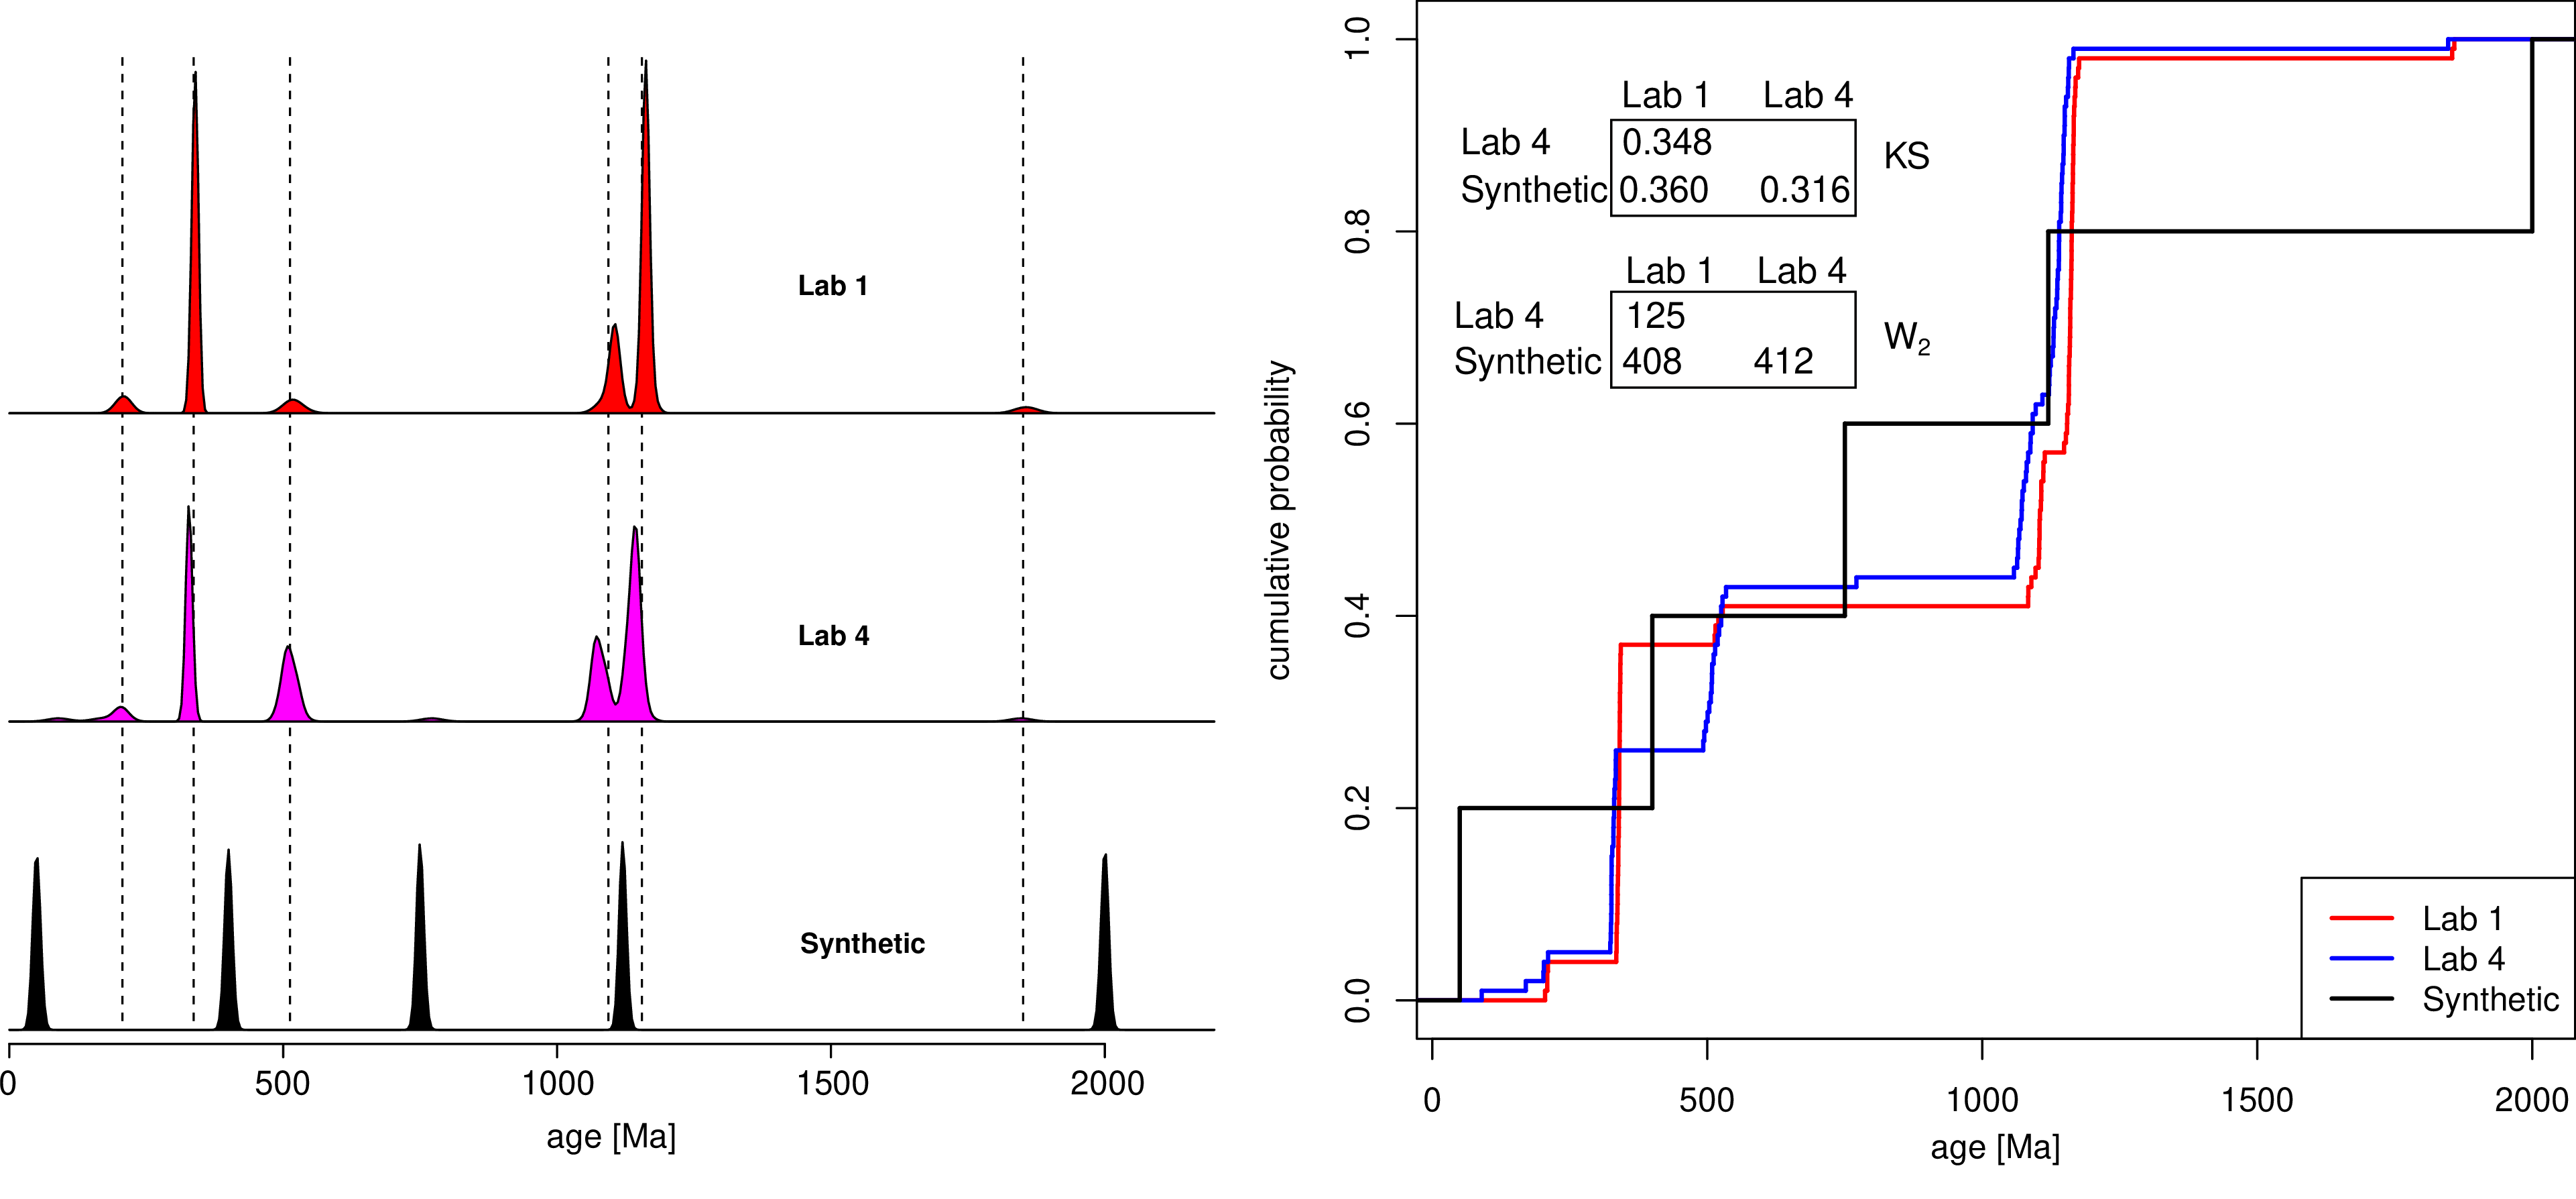
\includegraphics[width=\linewidth]{rev_figures/Kosler.pdf}
    \caption{\textbf{Comparing samples from an inter-laboratory calibration study}. KDEs (left) and ECDFs (right) of two samples from the inter-laboratory comparison study of \citep{kosler_u-pb_2013}, plus a purposefully misaligned synthetic sample. Dashed lines mark the true ages of the detrital mixture. According to the KS-statistic, the age distribution produced by Lab 4 is more similar to the synthetic distribution than it is to the distribution produced by Lab 1, despite the absence of any shared age components. The $W_2$ distance correctly deems the distribution produced by Lab~4 to be closer to that of Lab~1 than to the synthetic mixture.}
    \label{fig:interlab}
\end{figure}

A final scenario where the $W_2$ could be preferable is when comparing samples from different laboratories which are affected by inter-laboratory bias. \citet{kosler_u-pb_2013} provided ten different laboratories with identical synthetic zircon samples with a known age distribution. Different instruments introduced small differences in the ages of each peak. For example, in Figure \ref{fig:interlab} we display the results from Lab 1 (red) and Lab 4 (pink) as KDEs. The expected peak at $\sim$ 1200 Ma (dashed line) is offset between the two samples. As it is the maximum distance between two ECDFs, the KS distance is very sensitive to minor offsets in sharply defined peaks. In this case, the KS distance between these theoretically identical samples is large at 0.348, which is over one third of the maximum possible distance between samples. Indeed, the KS distance considers a synthetic, purposefully misaligned series of peaks (black KDE) to be more similar to the Lab 4 results than the results from Lab 1. The $W_2$ distance, does not suffer from this oversensitivity to minorly offset peaks and correctly identifies the samples from Lab 1 and Lab 4 as being much more similar than the random synthetic distribution.   

\section{Implementation} 

We provide example code (\DIFdelbegin %DIFDELCMD < \url{github.com/AlexLipp/detrital-wasserstein/}%%%
\DIFdelend \DIFaddbegin \href{https://github.com/AlexLipp/detrital-wasserstein}{\url{github.com/AlexLipp/detrital-wasserstein}}\DIFaddend ) in both \DIFdelbegin %DIFDELCMD < {\sf %%%
\DIFdel{python}%DIFDELCMD < } %%%
\DIFdel{and }%DIFDELCMD < {\sf %%%
\DIFdel{R }%DIFDELCMD < } %%%
\DIFdelend \DIFaddbegin \DIFadd{Python and R }\DIFaddend that demonstrates how to calculate the $W_2$ between two univariate distributions (U-Pb zircon ages). For these examples we make use of the the {\sf POT} and {\sf transport} packages in \DIFdelbegin \texttt{\DIFdel{python}} %DIFAUXCMD
\DIFdel{and }\texttt{\DIFdel{R}} %DIFAUXCMD
\DIFdelend \DIFaddbegin \DIFadd{Python and R }\DIFaddend respectively which implement solutions to Equation \ref{eq:def_1d} \citep{flamary_pot_2021,schuhmacher_transport_2022}.

\subsection{IsoplotR}

Additionally, the $W_2$-distance has been added to the \DIFdelbegin \texttt{\DIFdel{IsoplotR}} %DIFAUXCMD
\DIFdel{package in }\texttt{\DIFdel{R}}%DIFAUXCMD
\DIFdelend \DIFaddbegin \DIFadd{IsoplotR package in R}\DIFaddend , which calculates dissimilarity matrices and MDS maps \citep{vermeesch_isoplotr_2018}. This software can  be accessed using an (online) graphical user interface, at \DIFdelbegin %DIFDELCMD < \url{isoplotr.es.ucl.ac.uk}%%%
\DIFdelend \DIFaddbegin \href{https://isoplotr.es.ucl.ac.uk/}{\url{isoplotr.es.ucl.ac.uk}}\DIFaddend . Alternatively, the function can also be accessed from the \DIFdelbegin \texttt{\DIFdel{R}} %DIFAUXCMD
\DIFdelend \DIFaddbegin \DIFadd{R }\DIFaddend command line. The following snippet uses $W_2$ to calculate an MDS map for the dataset from \citet{wobus_has_2003} discussed in the manuscript (Figure \ref{fig:Wobus}). The data required is also available at the above repository. Note that the MDS map produced may show slight differences to those in the manuscript due to dependence of metric MDS on a random state variable. \DIFaddbegin \DIFadd{This variability can introduce reflections/rotations of the data, but the underlying structure is unchanged.
}\DIFaddend 

\DIFmodbegin
\begin{DIFverbatim}[alsolanguage=DIFcode]
# load the package:
library(IsoplotR)
%DIF > 
%DIF > # Load in the data 
DZ <- read.data("wobus.csv",method="detritals")
%DIF > 
# example 1. calculate the W2 distance matrix for the dataset:
d <- diss(DZ,method="W2") 
%DIF > 
# example 2. apply MDS to the dataset:
mds(DZ,method="W2")
\end{DIFverbatim}
\DIFmodend

\section{Conclusions}

The second Wasserstein distance, $W_2$, is an effective metric for comparing distributional data in the geological sciences such as detrital age spectra or grain size. Unlike the KS distance, $W_2$ can be extended to further dimensions. $W_2$ is a function of the horizontal distances between observations, in contrast to the KS distance, which corresponds to vertical differences between ECDFs. 
% We performed a case study in which eight zircon U-Pb age distributions from Scandinavian river sediments were analysed by MDS using $W_2$. We showed that the resulting MDS map accurately clusters samples with the same provenance together. Additionally, the relative positions of samples on the map coincide with trends in interpretable qualities such as distribution shape and average age.  
Using a variety of case studies we explore scenarios where the $W_2$ may or may not be preferable to the KS distance. In scenarios where discrete, known age peaks are mixed, the KS distance may be preferable. However, in other scenarios where absolute differences along the time axis are useful information, $W_2$ is preferable. Example scenarios include spatially/temporally evolving source distributions, thermochronological data, and combining detrital samples from different laboratories. The Wasserstein distance has been added to the \DIFdelbegin \texttt{\DIFdel{IsoplotR}} %DIFAUXCMD
\DIFdelend \DIFaddbegin \DIFadd{IsoplotR }\DIFaddend software, and example scripts are provided in \DIFdelbegin \texttt{\DIFdel{python}} %DIFAUXCMD
\DIFdel{and }\texttt{\DIFdel{R}}%DIFAUXCMD
\DIFdelend \DIFaddbegin \DIFadd{Python and R}\DIFaddend . 


%% The following commands are for the statements about the availability of data sets and/or software code corresponding to the manuscript.
%% It is strongly recommended to make use of these sections in case data sets and/or software code have been part of your research the article is based on.

\DIFdelbegin %DIFDELCMD < \codeavailability{The code and data repository is found at \url{https://github.com/AlexLipp/detrital-wasserstein}} %%%
\DIFdelend \DIFaddbegin \codeavailability{The code and data repository is found at \href{https://github.com/AlexLipp/detrital-wasserstein}{\url{github.com/AlexLipp/detrital-wasserstein}}} \DIFaddend %% use this section when having only software code available


\authorcontribution{AGL conceived the project, both authors contributed to development, writing, and software production.} %% this section is mandatory

\competinginterests{PV is an Associate Editor of Geochronology} %% this section is mandatory even if you declare that no competing interests are present

\begin{acknowledgements}

AGL is funded by a Junior Research Fellowship from Merton College, Oxford. PV is supported by NERC Standard Grant \#NE/T001518/1. This work benefited from discussions with Malcolm Sambridge \& Kerry Gallagher. We thank \DIFdelbegin \DIFdel{two anonymous reviewers}\DIFdelend \DIFaddbegin \DIFadd{reviews from Joel Saylor, an anonymous reviewer}\DIFaddend , and the associate editor Michael Dietze for their constructive feedback. 

\end{acknowledgements}




%% REFERENCES

%% The reference list is compiled as follows:

\bibliography{references.bib}

%% Since the Copernicus LaTeX package includes the BibTeX style file copernicus.bst,
%% authors experienced with BibTeX only have to include the following two lines:
%%
%% \bibliographystyle{copernicus}
%% \bibliography{example.bib}
%%
%% URLs and DOIs can be entered in your BibTeX file as:
%%
%% URL = {http://www.xyz.org/~jones/idx_g.htm}
%% DOI = {10.5194/xyz}


%% LITERATURE CITATIONS
%%
%% command                        & example result
%% \citet{jones90}|               & Jones et al. (1990)
%% \citep{jones90}|               & (Jones et al., 1990)
%% \citep{jones90,jones93}|       & (Jones et al., 1990, 1993)
%% \citep[p.~32]{jones90}|        & (Jones et al., 1990, p.~32)
%% \citep[e.g.,][]{jones90}|      & (e.g., Jones et al., 1990)
%% \citep[e.g.,][p.~32]{jones90}| & (e.g., Jones et al., 1990, p.~32)
%% \citeauthor{jones90}|          & Jones et al.
%% \citeyear{jones90}|            & 1990



%% FIGURES

%% When figures and tables are placed at the end of the MS (article in one-column style), please add \clearpage
%% between bibliography and first table and/or figure as well as between each table and/or figure.

% The figure files should be labelled correctly with Arabic numerals (e.g. fig01.jpg, fig02.png).


%% ONE-COLUMN FIGURES

%%f
%\begin{figure}[t]
%\includegraphics[width=8.3cm]{FILE NAME}
%\caption{TEXT}
%\end{figure}
%
%%% TWO-COLUMN FIGURES
%
%%f
%\begin{figure*}[t]
%\includegraphics[width=12cm]{FILE NAME}
%\caption{TEXT}
%\end{figure*}
%
%
%%% TABLES
%%%
%%% The different columns must be seperated with a & command and should
%%% end with \\ to identify the column brake.
%
%%% ONE-COLUMN TABLE
%
%%t
%\begin{table}[t]
%\caption{TEXT}
%\begin{tabular}{column = lcr}
%\tophline
%
%\middlehline
%
%\bottomhline
%\end{tabular}
%\belowtable{} % Table Footnotes
%\end{table}
%
%%% TWO-COLUMN TABLE
%
%%t
%\begin{table*}[t]
%\caption{TEXT}
%\begin{tabular}{column = lcr}
%\tophline
%
%\middlehline
%
%\bottomhline
%\end{tabular}
%\belowtable{} % Table Footnotes
%\end{table*}
%
%%% LANDSCAPE TABLE
%
%%t
%\begin{sidewaystable*}[t]
%\caption{TEXT}
%\begin{tabular}{column = lcr}
%\tophline
%
%\middlehline
%
%\bottomhline
%\end{tabular}
%\belowtable{} % Table Footnotes
%\end{sidewaystable*}
%
%
%%% MATHEMATICAL EXPRESSIONS
%
%%% All papers typeset by Copernicus Publications follow the math typesetting regulations
%%% given by the IUPAC Green Book (IUPAC: Quantities, Units and Symbols in Physical Chemistry,
%%% 2nd Edn., Blackwell Science, available at: http://old.iupac.org/publications/books/gbook/green_book_2ed.pdf, 1993).
%%%
%%% Physical quantities/variables are typeset in italic font (t for time, T for Temperature)
%%% Indices which are not defined are typeset in italic font (x, y, z, a, b, c)
%%% Items/objects which are defined are typeset in roman font (Car A, Car B)
%%% Descriptions/specifications which are defined by itself are typeset in roman font (abs, rel, ref, tot, net, ice)
%%% Abbreviations from 2 letters are typeset in roman font (RH, LAI)
%%% Vectors are identified in bold italic font using \vec{x}
%%% Matrices are identified in bold roman font
%%% Multiplication signs are typeset using the LaTeX commands \times (for vector products, grids, and exponential notations) or \cdot
%%% The character * should not be applied as mutliplication sign
%
%
%%% EQUATIONS
%
%%% Single-row equation
%
%\begin{equation}
%
%\end{equation}
%
%%% Multiline equation
%
%\begin{align}
%& 3 + 5 = 8\\
%& 3 + 5 = 8\\
%& 3 + 5 = 8
%\end{align}
%
%
%%% MATRICES
%
%\begin{matrix}
%x & y & z\\
%x & y & z\\
%x & y & z\\
%\end{matrix}
%
%
%%% ALGORITHM
%
%\begin{algorithm}
%\caption{...}
%\label{a1}
%\begin{algorithmic}
%...
%\end{algorithmic}
%\end{algorithm}
%
%
%%% CHEMICAL FORMULAS AND REACTIONS
%
%%% For formulas embedded in the text, please use \chem{}
%
%%% The reaction environment creates labels including the letter R, i.e. (R1), (R2), etc.
%
%\begin{reaction}
%%% \rightarrow should be used for normal (one-way) chemical reactions
%%% \rightleftharpoons should be used for equilibria
%%% \leftrightarrow should be used for resonance structures
%\end{reaction}
%
%
%%% PHYSICAL UNITS
%%%
%%% Please use \unit{} and apply the exponential notation


\end{document}
